\documentclass[conference,compsoc]{IEEEtran}

\usepackage[square,comma,numbers,sort&compress]{natbib}

% common packages
\usepackage{silence}
\WarningFilter*{caption}{Unsupported document class}

\usepackage[hyphens]{url}
\usepackage[breaklinks,colorlinks]{hyperref}
\usepackage[usenames,dvipsnames]{xcolor}
\hypersetup{citecolor=blue,linkcolor=blue}
\usepackage{amsmath,amsopn,amssymb}
\usepackage{subfig}
\usepackage{endnotes,microtype,xspace,graphicx,fancyvrb,multirow}
\usepackage{booktabs}
\usepackage{array,underscore,relsize}
\usepackage[T1]{fontenc}
\usepackage{times}
\usepackage{fancyhdr,lastpage}
\usepackage{enumitem}
\usepackage[labelfont=bf,font=small,skip=5pt]{caption}
\pagestyle{fancy}
\fancyhf{}
\renewcommand{\headrulewidth}{0pt}
\cfoot{\thepage}

% for math macro and numbers
\usepackage{fp}
\usepackage{siunitx}

% balance bibliography
\usepackage{balance}

% use \num{123456} -> 123,456
\sisetup{group-separator={,},group-minimum-digits={3},output-decimal-marker={.}}

\usepackage[flushleft]{threeparttable}

\usepackage{makecell}
\renewcommand{\theadalign}{l}

\usepackage{pifont}
\newcommand{\xmark}{\ding{55}}

\usepackage{mathrsfs}


%%% Local Variables:
%%% mode: latex
%%% TeX-master: "p"
%%% End:

\usepackage{kotex}

\newcommand{\sys}{\mbox{\textsc{C2Fuzz}}\xspace}

% ref. http://en.wikibooks.org/wiki/LaTeX/Colors
\newcommand{\BL}[1]{\textcolor{LimeGreen}{BL: #1}}
\newcommand{\yj}[1]{\textcolor{cyan}{YJ: #1}}
\newcommand{\dr}[1]{\textcolor{red}{DR: #1}}
\newcommand{\red}[1]{\textcolor{red}{#1}}
\newcommand{\XX}[0]{\textcolor{red}{XXX}}
\newcommand{\XXX}[1]{\textcolor{red}{XXX: #1}}
\newcommand{\TODO}[1]{\textcolor{Melon}{TODO: #1}}
\newcommand{\cutq}[1]{\textcolor{Melon}{CUT: #1}}
\newcommand{\cut}[1]{}

\renewcommand{\ttdefault}{pxtt}

\newcommand{\URL}{\url}
\newcommand{\cc}[1]{\mbox{\smaller[0.5]\texttt{#1}}}

% enable the below for ACM camera ready
%\clubpenalty=10000
%\widowpenalty=10000
%\renewcommand*{\bibfont}{\raggedright}

%\linespread{1.2}

\fvset{fontsize=\scriptsize,xleftmargin=8pt,numbers=left,numbersep=5pt}


\makeatletter
\def\PY@reset{\let\PY@it=\relax \let\PY@bf=\relax%
    \let\PY@ul=\relax \let\PY@tc=\relax%
    \let\PY@bc=\relax \let\PY@ff=\relax}
\def\PY@tok#1{\csname PY@tok@#1\endcsname}
\def\PY@toks#1+{\ifx\relax#1\empty\else%
    \PY@tok{#1}\expandafter\PY@toks\fi}
\def\PY@do#1{\PY@bc{\PY@tc{\PY@ul{%
    \PY@it{\PY@bf{\PY@ff{#1}}}}}}}
\def\PY#1#2{\PY@reset\PY@toks#1+\relax+\PY@do{#2}}

\@namedef{PY@tok@w}{\def\PY@tc##1{\textcolor[rgb]{0.73,0.73,0.73}{##1}}}
\@namedef{PY@tok@c}{\let\PY@it=\textit\def\PY@tc##1{\textcolor[rgb]{0.24,0.48,0.48}{##1}}}
\@namedef{PY@tok@cp}{\def\PY@tc##1{\textcolor[rgb]{0.61,0.40,0.00}{##1}}}
\@namedef{PY@tok@k}{\let\PY@bf=\textbf\def\PY@tc##1{\textcolor[rgb]{0.00,0.50,0.00}{##1}}}
\@namedef{PY@tok@kp}{\def\PY@tc##1{\textcolor[rgb]{0.00,0.50,0.00}{##1}}}
\@namedef{PY@tok@kt}{\def\PY@tc##1{\textcolor[rgb]{0.69,0.00,0.25}{##1}}}
\@namedef{PY@tok@o}{\def\PY@tc##1{\textcolor[rgb]{0.40,0.40,0.40}{##1}}}
\@namedef{PY@tok@ow}{\let\PY@bf=\textbf\def\PY@tc##1{\textcolor[rgb]{0.67,0.13,1.00}{##1}}}
\@namedef{PY@tok@nb}{\def\PY@tc##1{\textcolor[rgb]{0.00,0.50,0.00}{##1}}}
\@namedef{PY@tok@nf}{\def\PY@tc##1{\textcolor[rgb]{0.00,0.00,1.00}{##1}}}
\@namedef{PY@tok@nc}{\let\PY@bf=\textbf\def\PY@tc##1{\textcolor[rgb]{0.00,0.00,1.00}{##1}}}
\@namedef{PY@tok@nn}{\let\PY@bf=\textbf\def\PY@tc##1{\textcolor[rgb]{0.00,0.00,1.00}{##1}}}
\@namedef{PY@tok@ne}{\let\PY@bf=\textbf\def\PY@tc##1{\textcolor[rgb]{0.80,0.25,0.22}{##1}}}
\@namedef{PY@tok@nv}{\def\PY@tc##1{\textcolor[rgb]{0.10,0.09,0.49}{##1}}}
\@namedef{PY@tok@no}{\def\PY@tc##1{\textcolor[rgb]{0.53,0.00,0.00}{##1}}}
\@namedef{PY@tok@nl}{\def\PY@tc##1{\textcolor[rgb]{0.46,0.46,0.00}{##1}}}
\@namedef{PY@tok@ni}{\let\PY@bf=\textbf\def\PY@tc##1{\textcolor[rgb]{0.44,0.44,0.44}{##1}}}
\@namedef{PY@tok@na}{\def\PY@tc##1{\textcolor[rgb]{0.41,0.47,0.13}{##1}}}
\@namedef{PY@tok@nt}{\let\PY@bf=\textbf\def\PY@tc##1{\textcolor[rgb]{0.00,0.50,0.00}{##1}}}
\@namedef{PY@tok@nd}{\def\PY@tc##1{\textcolor[rgb]{0.67,0.13,1.00}{##1}}}
\@namedef{PY@tok@s}{\def\PY@tc##1{\textcolor[rgb]{0.73,0.13,0.13}{##1}}}
\@namedef{PY@tok@sd}{\let\PY@it=\textit\def\PY@tc##1{\textcolor[rgb]{0.73,0.13,0.13}{##1}}}
\@namedef{PY@tok@si}{\let\PY@bf=\textbf\def\PY@tc##1{\textcolor[rgb]{0.64,0.35,0.47}{##1}}}
\@namedef{PY@tok@se}{\let\PY@bf=\textbf\def\PY@tc##1{\textcolor[rgb]{0.67,0.36,0.12}{##1}}}
\@namedef{PY@tok@sr}{\def\PY@tc##1{\textcolor[rgb]{0.64,0.35,0.47}{##1}}}
\@namedef{PY@tok@ss}{\def\PY@tc##1{\textcolor[rgb]{0.10,0.09,0.49}{##1}}}
\@namedef{PY@tok@sx}{\def\PY@tc##1{\textcolor[rgb]{0.00,0.50,0.00}{##1}}}
\@namedef{PY@tok@m}{\def\PY@tc##1{\textcolor[rgb]{0.40,0.40,0.40}{##1}}}
\@namedef{PY@tok@gh}{\let\PY@bf=\textbf\def\PY@tc##1{\textcolor[rgb]{0.00,0.00,0.50}{##1}}}
\@namedef{PY@tok@gu}{\let\PY@bf=\textbf\def\PY@tc##1{\textcolor[rgb]{0.50,0.00,0.50}{##1}}}
\@namedef{PY@tok@gd}{\def\PY@tc##1{\textcolor[rgb]{0.63,0.00,0.00}{##1}}}
\@namedef{PY@tok@gi}{\def\PY@tc##1{\textcolor[rgb]{0.00,0.52,0.00}{##1}}}
\@namedef{PY@tok@gr}{\def\PY@tc##1{\textcolor[rgb]{0.89,0.00,0.00}{##1}}}
\@namedef{PY@tok@ge}{\let\PY@it=\textit}
\@namedef{PY@tok@gs}{\let\PY@bf=\textbf}
\@namedef{PY@tok@gp}{\let\PY@bf=\textbf\def\PY@tc##1{\textcolor[rgb]{0.00,0.00,0.50}{##1}}}
\@namedef{PY@tok@go}{\def\PY@tc##1{\textcolor[rgb]{0.44,0.44,0.44}{##1}}}
\@namedef{PY@tok@gt}{\def\PY@tc##1{\textcolor[rgb]{0.00,0.27,0.87}{##1}}}
\@namedef{PY@tok@err}{\def\PY@bc##1{{\setlength{\fboxsep}{\string -\fboxrule}\fcolorbox[rgb]{1.00,0.00,0.00}{1,1,1}{\strut ##1}}}}
\@namedef{PY@tok@kc}{\let\PY@bf=\textbf\def\PY@tc##1{\textcolor[rgb]{0.00,0.50,0.00}{##1}}}
\@namedef{PY@tok@kd}{\let\PY@bf=\textbf\def\PY@tc##1{\textcolor[rgb]{0.00,0.50,0.00}{##1}}}
\@namedef{PY@tok@kn}{\let\PY@bf=\textbf\def\PY@tc##1{\textcolor[rgb]{0.00,0.50,0.00}{##1}}}
\@namedef{PY@tok@kr}{\let\PY@bf=\textbf\def\PY@tc##1{\textcolor[rgb]{0.00,0.50,0.00}{##1}}}
\@namedef{PY@tok@bp}{\def\PY@tc##1{\textcolor[rgb]{0.00,0.50,0.00}{##1}}}
\@namedef{PY@tok@fm}{\def\PY@tc##1{\textcolor[rgb]{0.00,0.00,1.00}{##1}}}
\@namedef{PY@tok@vc}{\def\PY@tc##1{\textcolor[rgb]{0.10,0.09,0.49}{##1}}}
\@namedef{PY@tok@vg}{\def\PY@tc##1{\textcolor[rgb]{0.10,0.09,0.49}{##1}}}
\@namedef{PY@tok@vi}{\def\PY@tc##1{\textcolor[rgb]{0.10,0.09,0.49}{##1}}}
\@namedef{PY@tok@vm}{\def\PY@tc##1{\textcolor[rgb]{0.10,0.09,0.49}{##1}}}
\@namedef{PY@tok@sa}{\def\PY@tc##1{\textcolor[rgb]{0.73,0.13,0.13}{##1}}}
\@namedef{PY@tok@sb}{\def\PY@tc##1{\textcolor[rgb]{0.73,0.13,0.13}{##1}}}
\@namedef{PY@tok@sc}{\def\PY@tc##1{\textcolor[rgb]{0.73,0.13,0.13}{##1}}}
\@namedef{PY@tok@dl}{\def\PY@tc##1{\textcolor[rgb]{0.73,0.13,0.13}{##1}}}
\@namedef{PY@tok@s2}{\def\PY@tc##1{\textcolor[rgb]{0.73,0.13,0.13}{##1}}}
\@namedef{PY@tok@sh}{\def\PY@tc##1{\textcolor[rgb]{0.73,0.13,0.13}{##1}}}
\@namedef{PY@tok@s1}{\def\PY@tc##1{\textcolor[rgb]{0.73,0.13,0.13}{##1}}}
\@namedef{PY@tok@mb}{\def\PY@tc##1{\textcolor[rgb]{0.40,0.40,0.40}{##1}}}
\@namedef{PY@tok@mf}{\def\PY@tc##1{\textcolor[rgb]{0.40,0.40,0.40}{##1}}}
\@namedef{PY@tok@mh}{\def\PY@tc##1{\textcolor[rgb]{0.40,0.40,0.40}{##1}}}
\@namedef{PY@tok@mi}{\def\PY@tc##1{\textcolor[rgb]{0.40,0.40,0.40}{##1}}}
\@namedef{PY@tok@il}{\def\PY@tc##1{\textcolor[rgb]{0.40,0.40,0.40}{##1}}}
\@namedef{PY@tok@mo}{\def\PY@tc##1{\textcolor[rgb]{0.40,0.40,0.40}{##1}}}
\@namedef{PY@tok@ch}{\let\PY@it=\textit\def\PY@tc##1{\textcolor[rgb]{0.24,0.48,0.48}{##1}}}
\@namedef{PY@tok@cm}{\let\PY@it=\textit\def\PY@tc##1{\textcolor[rgb]{0.24,0.48,0.48}{##1}}}
\@namedef{PY@tok@cpf}{\let\PY@it=\textit\def\PY@tc##1{\textcolor[rgb]{0.24,0.48,0.48}{##1}}}
\@namedef{PY@tok@c1}{\let\PY@it=\textit\def\PY@tc##1{\textcolor[rgb]{0.24,0.48,0.48}{##1}}}
\@namedef{PY@tok@cs}{\let\PY@it=\textit\def\PY@tc##1{\textcolor[rgb]{0.24,0.48,0.48}{##1}}}

\def\PYZbs{\char`\\}
\def\PYZus{\char`\_}
\def\PYZob{\char`\{}
\def\PYZcb{\char`\}}
\def\PYZca{\char`\^}
\def\PYZam{\char`\&}
\def\PYZlt{\char`\<}
\def\PYZgt{\char`\>}
\def\PYZsh{\char`\#}
\def\PYZpc{\char`\%}
\def\PYZdl{\char`\$}
\def\PYZhy{\char`\-}
\def\PYZsq{\char`\'}
\def\PYZdq{\char`\"}
\def\PYZti{\char`\~}
% for compatibility with earlier versions
\def\PYZat{@}
\def\PYZlb{[}
\def\PYZrb{]}
\makeatother


\newcommand{\figrule}{\hrule width \hsize height .33pt}
\newcommand{\coderule}{\vspace{-0.5em}\figrule\vspace{0.2em}}

\setlength{\abovedisplayskip}{0pt}
\setlength{\abovedisplayshortskip}{0pt}
\setlength{\belowdisplayskip}{0pt}
\setlength{\belowdisplayshortskip}{0pt}
\setlength{\jot}{0pt}

\def\Snospace~{\S{}}
\renewcommand*\sectionautorefname{\Snospace}
\def\sectionautorefname{\Snospace}
\def\subsectionautorefname{\Snospace}
\def\subsubsectionautorefname{\Snospace}
\def\chapterautorefname{\Snospace}
%\renewcommand{\figurename}{Fig.}
%\def\figureautorefname{\figurename}
\newcommand{\subfigureautorefname}{\figureautorefname}

%\numberwithin{equation}{section}
\newcommand{\yes}{Y}
\newcommand{\no}{}

% sema
\newcommand{\shl}{\ \cc{<}\cc{<}\ }
\newcommand{\shr}{\ \cc{>}\cc{>}\ }
\newcommand{\x}{$\times$\xspace}

\if 0
\renewcommand{\topfraction}{0.9}
\renewcommand{\dbltopfraction}{0.9}
\renewcommand{\bottomfraction}{0.8}
\renewcommand{\textfraction}{0.05}
\renewcommand{\floatpagefraction}{0.9}
\renewcommand{\dblfloatpagefraction}{0.9}
\setcounter{topnumber}{10}
\setcounter{bottomnumber}{10}
\setcounter{totalnumber}{10}
\setcounter{dbltopnumber}{10}
\fi

\newif\ifdraft\drafttrue
\newif\ifnotes\notestrue
\ifdraft\else\notesfalse\fi

% hide comments
% \renewcommand{\TK}[1]{\ignorespaces}
% \renewcommand{\XXX}[1]{\ignorespaces}
% \renewcommand{\TODO}[1]{\ignorespaces}

%% Ensure ligatures (e.g., ``fine official flag'') can be copy/pasted from PDF.
\input{glyphtounicode}
\pdfgentounicode=1

\newcolumntype{R}[1]{>{\raggedleft\let\newline\\\arraybackslash\hspace{0pt}}p{#1}}

% include macros
\newcommand{\includepdf}[1]{
  \includegraphics[width=\columnwidth]{#1}
}
\newcommand{\includeplot}[1]{
  \resizebox{\columnwidth}{!}{\input{#1}}
}

% list
\newcommand{\squishlist}{
\begin{itemize}[noitemsep,nolistsep]
  \setlength{\itemsep}{-0pt}
}
\newcommand{\squishend}{
  \end{itemize}
}

%%
%% NOTE.
%%  to use circled number in caption, use
%%   (e.g., \protect\C{1})
%%
\usepackage{tikz}
\newcommand*\C[1]{%
\begin{tikzpicture}[baseline=(C.base)]
\node[draw,circle,inner sep=0.2pt](C) {#1};
\end{tikzpicture}}

\newcommand*\BC[1]{%
\begin{tikzpicture}[baseline=(C.base)]
\node[draw,circle,fill=black,inner sep=0.2pt](C) {\textcolor{white}{#1}};
\end{tikzpicture}
}

\usepackage{xstring}
\newcommand{\PP}[1]{
\vspace{2px}
\noindent{\bf \IfEndWith{#1}{.}{#1}{#1.}}
}

\newcommand{\ra}[1]{\renewcommand{\arraystretch}{#1}}
\newcommand{\V}{\checkmark}
\newcommand{\X}{{\footnotesize $\times$}\xspace}
\renewcommand{\O}{\phantom{0}}

%% units
\newcommand{\B}{\,\text{B}\xspace}
\newcommand{\K}{\,\text{K}\xspace}
\newcommand{\M}{\,\text{M}\xspace}
\newcommand{\T}{\,\text{T}\xspace}
\newcommand{\KB}{\,\text{KB}\xspace}
\newcommand{\MB}{\,\text{MB}\xspace}
\newcommand{\GB}{\,\text{GB}\xspace}
\newcommand{\TB}{\,\text{TB}\xspace}

\newcommand{\Bs}{\,\text{B/s}\xspace}
\newcommand{\KBs}{\,\text{KB/s}\xspace}
\newcommand{\MBs}{\,\text{MB/s}\xspace}
\newcommand{\GBs}{\,\text{GB/s}\xspace}

\newcommand{\etal}{\textit{et al}.\xspace}
\newcommand{\ie}{\textit{i}.\textit{e}.}
\newcommand{\eg}{\textit{e}.\textit{g}.}

\newcommand{\totalbugs}{17\xspace}
\newcommand{\studiedbugs}{15\xspace}

%%% Local Variables:
%%% mode: latex
%%% TeX-master: "p"
%%% End:

\IfFileExists{rev.tex}{\gdef\therev{097b76f}
\gdef\thedate{2022-08-02 19:34:47 +0900}
}{}

\begin{document}

\title{\sys: Segmentizing Thread Interleaving to Find Kernel Concurrency Bugs through Fuzzing}

% when 'make draft'
\ifdefined\DRAFT
 \pagestyle{fancyplain}
 \lhead{Rev.~\therev}
 \rhead{\thedate}
 \cfoot{\thepage\ of \pageref{LastPage}}
\fi

% blind
% \author{Paper \#123}


\author{
  Paper \#2
}


%%% Local Variables:
%%% mode: latex
%%% TeX-master: "p"
%%% End:

\date{}
\maketitle

\thispagestyle{plain}
\pagestyle{plain}

\begin{abstract}
\sys
\end{abstract}

%%% Local Variables:
%%% mode: latex
%%% TeX-master: "p"
%%% End:

\section{Introduction}
\label{s:intro}

%\dr{I make a decision to denote ``(thread) interleaving'' as a whole
%  interleaving. MUZZ and Krace use the term like this.}

Concurrency bugs are common in modern kernels due to 
the pervasive adoption of efficient but difficult-to-reason
parallelization techniques.
The consequence of kernel concurrency bugs is disastrous. They crash
the entire system, breaking availability~\cite{cve201812232, snowboardbug} or causing data loss~\cite{dataloss}.
Furthermore, attackers 
exploit concurrency bugs to mount a privilege escalation attack.
A recent study~\cite{exprace} demonstrates that a user-level attacker 
reliably exploits non-deterministic concurrency bugs without performing
brute-force attacks.

Identifying kernel concurrency bugs is much more difficult than 
finding non-concurrency bugs. 
In contrast to non-concurrency bugs which are identified by 
sequential testing of a single thread execution,
kernel concurrency bugs are typically caused by the concurrent execution 
of two or more threads.
Kernel concurrency bugs only emerge in a particular pattern of 
interleavings between threads. The thread interleaving happens 
rarely because it takes place only when a certain timing condition is met.
Unfortunately, to discover concurrency bugs, exploring all the possible interleavings is not practical because 
the number of instructions executed by a system call in Linux is huge.
%Due to such difficulty, traditional fuzzers..

%\dr{as far as I know, there are conzzer and muzz}
%\dr{If we consider Snowboard as a fuzzer, Snowboard does not
%  adopt an interleaving coverage metric, so it cannot distinguish two
%  interleavings, and it relies on *heuristics* (= clustering
%  strategies) to determine which interleavings should be explored}
To increase efficiency of concurrency bug fuzzing, several approaches
have been proposed. \yj{how to put SKI?}\dr{we don't need to. It is not a fuzzer} Razzer~\cite{razzer} uses static analysis to 
identify memory-accessing instruction pairs of the same objects, and 
Snowboard~\cite{snowboard} uses dynamic analysis. 
From the detected instruction pairs, they perform randomized 
scheduling to generate new thread interleavings. Alas,
the randomized exploration are inefficient to explore the large 
thread interleaving search space. Instead, we emphasize that 
coverage-guided searching would be more preferable strategy 
for concurrency fuzzing. however, it is not well-studied that 
what form of coverage would be efficient in concurrency fuzzing.
KRACE~\cite{krace} proposes alias coverage, which simply tracks 
a single alias pair instruction. We observe that tracking single 
instruction pairs are not sufficient. Furthermore, KRACE uses 
the alias coverage to decide continuing to explore or not 
in the current multi-thread input. When exploring the thread 
interleaving space, it also take a similar randomized approach, 
sharing the similar inefficiency of previous techniques.


To overcome the shortcoming of existing methods, this paper proposes
\sys, a fuzzing framework for kernel concurrency bugs. 
\sys discovers not only data races but 
all interleaving-related bugs. 
At its core, \sys aims to systematically explore the vast thread
interleaving search space to quickly identify the multi-thread input and 
interleavings leading to a concurrency bug. The central idea behind \sys's design
is i) defining a new, effective coverage metric that reflects the 
common nature of concurrency bugs and ii) use that metric to drive 
an efficient search strategy for discovering previously untested interleavings.
Hence, we demonstrate that \sys saves a significant amount of CPU expenses 
in large-scale fuzzing by fast finding concurrent bugs, 
without sacrificing bug-detecting capability (sometimes having better 
capability than earlier work).
\sys achieves the goal with the following two key ideas: segmentizing thread interleaving and speculative exploration  of interleavings.

\PP{Segmentizing thread interleaving} From the execution of two threads,  
\sys decomposes the large thread interleaving space into tractable 
small sub-spaces, called \textit{interleaving segment} in which
instructions access shared memory objects. The number of instructions 
in a segment is small (at most four by default), and each segment may 
contain multiple interleavings. Using interleaving segments, we propose 
our new coverage metric, \textit{\intcov}, defined as a set of detected segments. \Intcov generalizes coverage 
metrics proposed by previous approaches where they only tracks 
a single interleaving (the size of a segment is 2)\yj{OK?}. 
Using \intcov provides two benefits to fuzzers. First, a fuzzer can 
take into account the interactions of multiple interleavings, which increases
accuracy of discovering concurrency bugs in comparison to considering a single 
interleavings. A previous study~\cite{learningfrommistakes} identifies that
most concurrency bugs occurs by multiple interleavings involving 
at most four memory accesses of shared memory objects.
Second, using \intcov, a fuzzer can produce a thread interleaving
that have not yet been found for the subsequent search.

\PP{Speculative exploration of interleavings} \yj{Speculative exploration
  might be a misleading term}
%
\dr{I don't get a point. I think it is a proper term because we
  speculate mutated segments, then check that they are executable
  (some of them are not executable because of lock or race-steered
  control flow).}
%
To explore new interleavings,
\sys mutates observed interleavings recorded in \intcov. For mutating a segment, \sys changes interleaving orders of observed interleavings 
in a segment, which generates new interleavings for testing. \sys 
mutates as many segments as possible in the expectation that the 
new interleavings include a large number of untested interleavings. 
This search strategy quickly navigates the search space than previous 
approaches in which only one interleaving is mutated at each search step

We implement \sys across various software layers.
We extend Syzkaller~\cite{syzkaller} to generate concurrency fuzzing inputs 
and segment mutations. 
%
In addition, \sys incorporates a LLVM pass to transform a kernel
binary for tracking \intcov, and the QEMU/KVM-based execution engine
to enforce thread scheduling obtained by segment mutations. 
%
We run \sys against the latest version of the Linux kernel (ranging
from 5.19-rc2 to 6.0-rc7), and find new \totalbugs concurrency bugs all of
which exhibits harmful behaviors such as memory corruption,
task hangs, or assertion violations. We emphasize that all
concurrency bugs found by \sys were lurking in subsystems where
Syzkaller~\cite{syzkaller} has been testing for several years, which
demonstrates the usefulness of \sys in bug-finding capability.
%
To quantify the efficiency of \sys, we experimentally compare \sys 
against the state-of-the-art techniques, Snowboard and KRACE and 
demonstrate that \sys discover concurrency bugs more quickly 
(up to \yj{xx}$\times$) than previous work using the segment mutation 
technique.

We describe our contributions in three folds:

\begin{itemize}
\item interleaving segment coverage
\item speculative interleaving exploration based on explored interleaving
\item We have found \totalbugs race conditions.
\end{itemize}

%%% Local Variables:
%%% mode: latex
%%% TeX-master: "p"
%%% End:

\section{Background}
\label{s:background}

While concurrency has been a cornerstone of performance benefits in
the multicore era, it leaves a risk of malfunction, \ie, concurrency
bug, caused by insufficient thought of concurrent events.
%
In this section, we describe two types of concurrency bug, data race
and race condition, and introduce prior approaches to spot out
concurrency bugs.

\subsection{Concurrency Bug}
\label{ss:concurrencybugs}

A concurrency bug can be classified into two categories according to
how it adversely affects a program.

\begin{figure}
  \centering
  \subfloat[Data race.\label{subfig:datarace}] {
    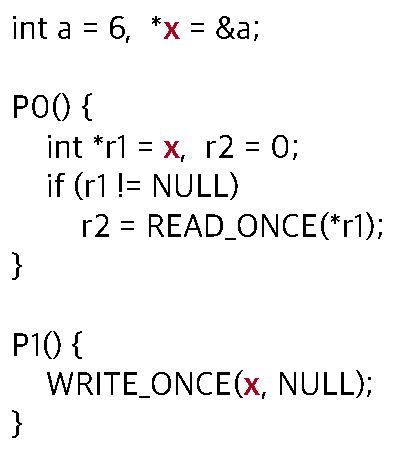
\includegraphics[width=0.45\linewidth]{fig/datarace.pdf}
  }
  \hfill
  \subfloat[Race condition.\label{subfig:racecondition}] {
    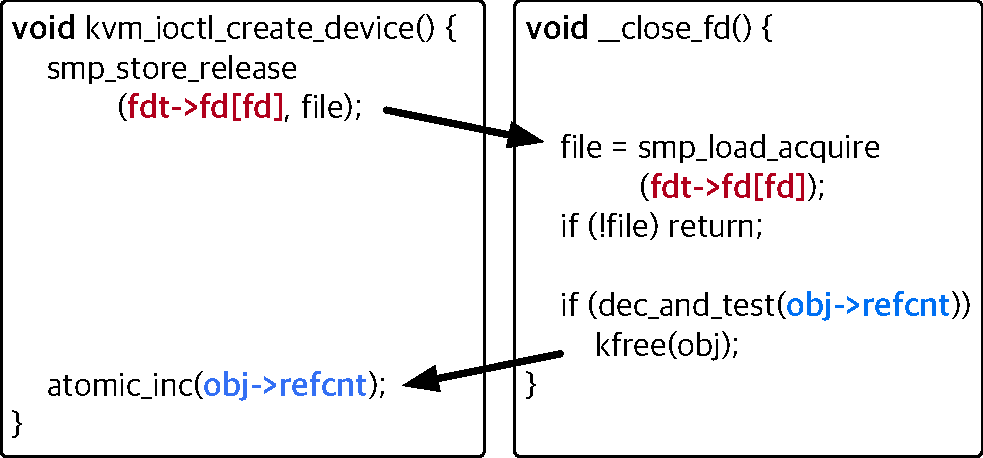
\includegraphics[width=0.45\linewidth]{fig/racecondition.pdf}
  }
  \caption{Two types of concurrency bugs.}
  \label{fig:concurrencybugs}
\end{figure}  


\PP{Data race.}
%
Although the concept of data race is well known, its formal definition
depends on a programming language~\cite{C-standard-n2310,
  java-standard} or a program in development~\cite{lkmm}. In this
paper, we employ the definition from Linux Kernel Memory Model
(LKMM)~\cite{lkmm}. According to LKMM, a data race occurs when there
are two memory accesses such that 1) they access the same location, 2)
at least one of them is a store, 3) at least one of them is not
annotated with special operations such as \texttt{WRITE_ONCE()}, or
\texttt{smp_load_acquire()}, 4) they occur on different CPUs (or in
different threads on the same CPU), and 5) they execute concurrently.
%
Informally, a data race indicates un-annotated concurrent accesses to
a shared memory location.

Data races are problematic because they may confuse a compiler.  LKMM
allows a compiler to assume that there will be no data race during the
runtime. Based on the assumption, a compiler has its rights to
arbitrarily transform plain accesses (\ie, accesses not annotated with
above operations), making the results unpredictable if there is a data
race during the runtime.
%
Therefore, LKMM defines the outcome of the program as undefined
behavior if a data race occurs.
%
Also, to prevent such undefined behaviors, LKMM requires developers to
annotate accesses if they possibly run
concurrently~\cite{data-race-fix1, data-race-fix2, data-race-fix3}.
% %
% On the other hand, data races may or may not cause a real-world issue
% such as memory corruption. Many data races fixes~\cite{data-race-fix1,
%   data-race-fix2, data-race-fix3} annotate memory accessing
% instructions with above operations, which actually does not affect the
% compiled binary.


\PP{Race condition.}
%
Race condition is another type of concurrency bug. While a race
condition broadly indicates that an outcome differs depending on the
timing of concurrent events, we restrict the definition to indicate
the correctness of the outcome differs according to the timing of
concurrent events.
%
Specifically, if developers do not take consider of all possible
interleavings, a program may execute an erroneous interleaving which
leads the program into an unintended state.
%
Immediately or after a certain amount of time, the unintended state
causes erroneous behaviors of the program such as memory corruption,
deadlock, and assertion violation.

% \dr{TODO: what more?}
% In order to fix the errorneous interelaving, developers often utilize
% synchronization primitives such as a lock, or switch the order of
% instructions in a program~\cite{learningfrommistakes}.


% https://stackoverflow.com/questions/11276259/are-data-races-and-race-condition-actually-the-same-thing-in-context-of-conc
%
\PP{Differences between data race and race condition}
%
\dr{TODO: rewrite to enphasize that finding race condition is
  important and combine this into the race condition paragraph}
%
Although both race condition and data race are a bug caused by
concurrenct events, there are a few differences.
%
First, a data race is regards to a single pair of conflicting accesses
while a race condition is about an interleaving.
%
Therefore, methods to detect them are also different.  While data race
detectors~\cite{tsan, krace, prorace, crsampler, txrace} monitor
whether two conflicting plain accesses are executed concurrently, race
conditions can be observed only through an erroneous behavior caused
by a specific interleaving.
%
Second, whereas a data race occurs if such conflicting accesses exists
no matter it causes an erroneous behavior or not, a race condition is
told by an abnormal outcome of a program.
%
% In the security perspective, a data race requires further
% investigation to determine whether it is harmful or
% not~\cite{portend, replayanalysis}, the effect of a race condition
% is exmained by erroneous behaviors such as general protection fault,
% assertion violations, sanitizers~\cite{asan, kasan} and
% lockdep~\cite{lockdep} reports.
%
% \begin{figure}
%   \centering
%   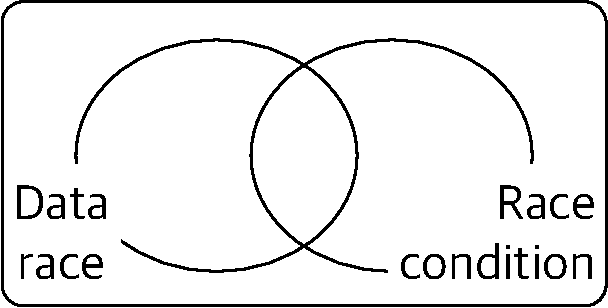
\includegraphics[width=0.45\linewidth]{fig/venndiagram.pdf}
%   \caption{Relation between data race and race condition. This paper
%     focuses on the striped region. \dr{I don't think we need this.}}
%   \label{fig:venndiagram}
% \end{figure}  
%
Lastly, they are not a subset or a superset of one another. Although
there are race conditions that occur with data races, neither one is
the sufficient nor necessary condition for the other. Therefore, we
would argue that finding data races and finding race condditions are
complementary with each other.


\PP{Scope of this paper}
%
This paper focuses on finding race conditions instead of data races.

\dr{TODO: why? want to say finding race condition is more important,
  and existing approaches to find data races are limited}

\dr{TODO: need to say the importance of observing erroneous outcomes}


\subsection{Concurrency Fuzzing}
\label{ss:concurrencyfuzzing}


% During fuzzing, a fuzzer determines that interleavings of given
% concurrent jobs are tested enough if a concurrency coverage is
% saturated while a customized scheduler is introduced to tailor the
% non-deterministic behavior.


In spite of enormous efforts, finding concurrency bugs is still a
daunting task.
%
It is mainly due to two challenges such that 1) concurrency bugs are
inherently caused non-deterministically, and 2) the number of possible
interleavings grows exponentially to the number of memory access
operations.

Recently, several studies~\cite{razzer, krace, snowboard, muzz} have
been proposed to improve fuzzing techniques specifically in exposing
concurrency bugs.
%
These studies generally adopt two strategies, namely customized
scheduler to tail the non-determinism, and coverage metric in the
concurrency dimension to capture interesting interleavings among all
possible interleavings.

\PP{Coverage-guided fuzzing}
%
Throughout decades, a fuzzing has shown its ability to find bugs in
various software layers including the userprogram space~\cite{qsym,
  driller, symsan, crfuzz, r2z2, cafl, fuzzorigin} and the kernel
space~\cite{fuzzusb, syzkaller, hfl, cabfuzz, razzer, krace, janus,
  hydra, healer}.
%
A primary task of fuzzing is to synthesize and mutate various inputs
of a target program.
%
When running the inputs, a fuzzer monitors a program's behavior, and
observes malfunctions with a help of various developer
tools~\cite{asan, kasan, meds}.

A coverage-guided fuzzer adopts a coverage metric to abstract
program's interesting behaviors.
%
During fuzzing, a fuzzer accumulates all experienced coverage as the
abstraction of tested behaviors of a program.
%
When a new input is given, a fuzzer compares coverage of the input
with the accumulated coverage to determine whether the input exposes a
new interesting behavior. If it does, a fuzzer keeps and mutates the
input to generate another input that potentially exhibits unknown
coverage.

% \dr{TODO: Do we need to tell about coverage-directed fuzzers?}

\PP{Customized scheduler.}
%
Instead of relying on the uncontrollable kernel scheduler, concurrency
fuzzing generally consists of a customized scheduler to increase the
probability of bugs being exposed.
%
Depending on how a customized scheduler schedules instructions, it is
largely categorized into randomized scheduler and scheduling
hint-directed scheduler (shortly, hint-directed scheduler).

A randomized scheduler~\cite{ski, pctalgorithm, krace, sparsernr} is
designed to randomly schedule intstructions in a disciplined
manner. It tries to keep only one thread to execute while the thread
runs until a certain number of instructions are executed or a certain
amount of time has elapsed.
%
A fuzzer and the scheduler share a small number of parameters used for
the scheduler to pseudo-randomly determine the number of instructions
or the amount of time to execute.
%
In this way, interleavings are diversified across fuzzing runs while a
fuzzer can tailor the non-determinism caused by scheduling.

On the other side, a hint-directed scheduler~\cite{razzer, snowboard}
enfoces a specific requirement of interleaving called a scheduling
hint.
%
A scheduling hint is generally in the form of an interleaving pattern
that possibly causes a concurrency bug. For example, a scheduling hint
may consists of execution order indicating a single-variable order
violation; \textit{``thread A executes a store operation writing into
  $X$ before thread B executes a load operation reading from $X$''}.
%
During fuzzing, a fuzzer keeps generating different scheduling hints,
and enforces an interleaving that contains a scheduling hint to
observe the interleaving causes an erroneous behavior.


\PP{Coverage in the concurrency dimension.}
%
To the best of our knowledge, Krace~\cite{krace} is the first work
that asserts the necessity of a coverage metric in the concurrency
dimension.
%
While many coverage metrics are proposed with their own pros and
cons~\cite{wang2019sensitive}, they only track the sequential aspect
of a program (\eg, branch coverage tracks whether a branch is taken or
not) without paying attention to communication between threads.
%
Krace states that even after sequential coverage is saturated, there
could be more interesting behaviors caused by thread interleavings,
and that if there are unexplored thread interleavings in an input, a
fuzzer should keep paying attention to the input.

To capture unique behaviors in the concurrency dimension, Krace
proposes a coverage metric called alias coverage.
%
Alias coverage tracks inter-thread data flow between a pair of
instructions. In other words, alias coverage tracks
\texttt{$I_S \rightarrow I_L$} if a load instruction \texttt{$I_L$}
reads a value written by a store instruction \texttt{$I_S$} and they
are executed in different threads.
%
% For example, if a fuzzer wants to test an interleaving that , it can
% instruct a scheduler to enfore such requirement on the two
% instructions.
%
\dr{TODO: MUZZ, and others?}
%
Although Razzer~\cite{razzer} and Snowboard~\cite{snowboard} adopt a
hint-directed scheduler, they do not make use of a concurrency
coverage metric. Therefore they do not distinguish whether two inputs
exhibit different behaviors. Instead, they concentrate on less
frequent inter-thread data flow based on an idea that those
inter-thread data flow is less likely tested and more likely causes an
abnormal behavior.

\section{Motivation}
\label{ss:motivation}

% - Coverage-guide fuzzing is important
% - How to define coverage in concurrency dimension is 
% challenging and important
% - Limitation of previous work: does not reflect 
% the nature of manifestation of race condition.

This work is motivated by an observation that prior approaches
focus on the execution order of a single pair of conflicting
accesses, but race conditions mostly are \textit{combined results of multiple pairs} 
of conflicting accesses.
%
Because of this gap\yj{xx}, prior approaches shows inefficiency in finding race
conditions.

In this section, we first describe when and how concurrency bugs
manifest to comprehend what interleavings should be tested to find
race conditions.
%
Afterwards, we identify why prior approaches are limited in finding
race conditions, and clarify our goals to address the limitations.


\PP{Manifestation of race conditions}
%
According to an extensive survey of concurrency
bugs~\cite{learningfrommistakes}, most race conditions manifest
depending on the execution order of multiple memory access operations.
%
Specifically, the study identifies that 92\% of race conditions manifest 
when at most four memory accesses operations are executed in a specific
order.
%
% For all other memory accesses, their execution orders and values
% written and read by them do not affect bugs's manifestation.

\begin{figure}[t]
  \centering
  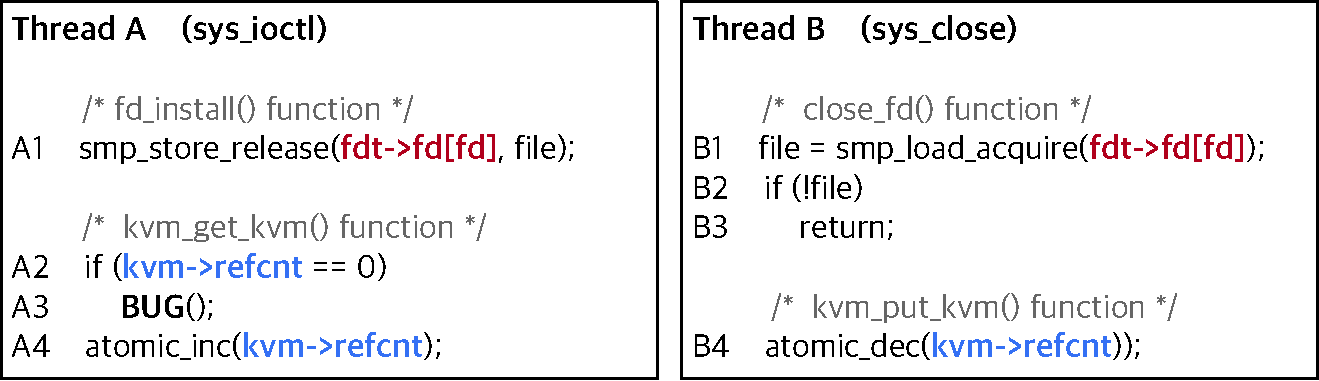
\includegraphics[width=0.95\linewidth]{fig/cve-2017-10661.pdf}
  \caption{Simplified code snippet of a NULL-dereference bug in the
    binder driver.}
  \label{fig:cve-2019-6974}
\end{figure}

\autoref{fig:cve-2019-6974} explains a case. In this example, a race
condition occurs in the binder device driver, which is an IPC
framework for Android. Specifically, a NULL-dereference bug manifests
when two system calls are executed concurrently: \texttt{mmap()} to
map the device driver into a user address space and
\texttt{ioctl(TRANSACTION)} to send an IPC message.


\yj{Are you talking about \autoref{fig:alias-coverage}?}
The race condition happens as follows. Let us suppose
\texttt{alloc->vma} and \texttt{alloc->mm} are initially
\texttt{NULL}.
%
During mapping the device driver into a user address space, thread~A
sets \texttt{alloc->vma} and \texttt{alloc->mm} to non-NULL pointers
at \texttt{A1} and \texttt{A2}.
%
However, since these two store operations are not atomically executed,
thread~B may intervene in the middle of these two instructions.
%
In that case, it is possible that \texttt{alloc->vma} is not
\texttt{NULL} when thread~B executes \texttt{B1} while
\texttt{alloc->mm} is \texttt{NULL} at \texttt{B4}.
%
As a consequnce, a NULL-dereference manifests when thread~B increments
the reference counter of \texttt{alloc->mm} at \texttt{B4}.
%
In summary, the manifestation of the race condition depends on whether
the execution order of four memory accesses meets a certain condition,
namely
$(\texttt{A1} \rightarrow \texttt{B1}) \wedge (\texttt{B4} \rightarrow
\texttt{A2})$~\footnote{In this paper, $X \rightarrow Y$ indicates that $X$
  is executed before $Y$}.

% One of the factors that makes it difficult to find concurrency bugs is
% that, they may be detected only when a program shows an abnormal
% behavior.
% %
% \autoref{subfig:racecondition} is the example of such concurrency bug.
% %
% In this example, the timing of accesses are not correctly
% contemplated. When instructions are executed in the order of
% \dr{TODO:}..., the program runs differently than the developer
% intention, causing a use-after-free bug.
% %
% However there are no plain accesses (\ie, all accesses are annotated),
% and therefore, there is no data race.
% %
% By the definition, data race detectors~\cite{tsan, kcsan, krace,
%   prorace, txrace, crsampler} are not applicable to detect this kind
% of race conditions.


% In worse cases, race conditions hardly manifest with the kernel
% scheduler. In detail, a race condition may manifest only when one
% thread stalls for a long time while another thread executes numerous
% instructions.
% %
% One could argue that those concurrency bugs are not a threat because
% it may take too long time, or even impossible to exploit.
% %
% However, a recent study, ExpRace~\cite{exprace}, reveals that an
% attacker can affect the kernel's scheduler using inter-processor
% interrupts (IPI), and exploit even such concurrency bugs.



\PP{Limitation of existing approaches}
%
In the perspective of fuzzing, a coverage metric is a paramount gear
to determine whether a given input is worthy of further mutation.
%
If a coverage metric does not represent whether an input has a
potential to trigger a race condition, a fuzzer may ignore inputs in
which there are unexplored interleavings, or waste the computing power
to valueless inputs.
%
In this regard, our primary question is whether existing coverage
metrics in the concurrency dimension are suitable to apprehend
interleavings potentially causing a race condition, for example,
$(\texttt{A1} \rightarrow \texttt{B1}) \wedge (\texttt{B4} \rightarrow
\texttt{A2})$ in \autoref{fig:cve-2019-6974}.



Unfortunately, we observe that none of existing approaches incorporate
a proper coverage metric for race conditions.
%
A few of existing approaches~\cite{snowboard, razzer} do not adopt a
coverage in the concurrency dimension at all. Therefore, they do not
make a decision as to whether a given input is worth further testing.
%
Other approaches~\cite{krace, muzz} adopt coverage metrics that are
not suitable for race conditions as they do not consider a combined
result of multiple pairs of conflicting accesses. As a consequence,
race conditions may not be exposed even after the coverages are
saturated.
%
% Consequently, existing approaches have difficulty in distinguishing a
% given input has a potential to cause an interesting behavior, \ie,
% a race condition.


\begin{figure}[t]
  \centering
  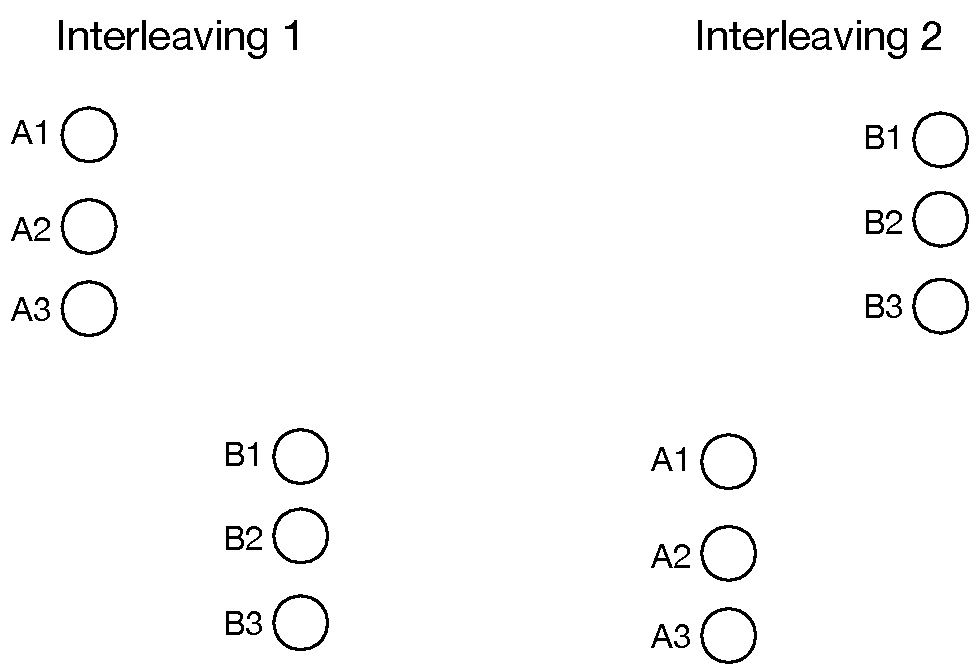
\includegraphics[width=0.98\linewidth]{fig/alias-coverage.pdf}
  \caption{Three inputs that consist of two concurrent syscalls. For
    all inputs, thread~A executes the same \texttt{mmap()} syscall
    while thread~B handles different ioctl requests. For brevity, we
    describe only conflicting instructions.}
  \label{fig:alias-coverage}
\end{figure}

\yj{This is the key paragraph to point out the limitation of previous approaches, but very vague. Make specific claims of why Kraces' alias coverage is insufficient by giving an example.}
%
In order to show why comprehending multiple pairs of conflicting
accesses is important, let us suppose we have three inputs that
consists of two concurrent syscalls as described in
\autoref{fig:alias-coverage}.
%
For all inputs, thread~A executes a \texttt{mmap()} syscall to map the
binder driver to a user address space while thread~B handles different
ioctl requests such that \texttt{ioctl(FREE_BUFFER)},
\texttt{ioctl(REPLY)}, and \texttt{ioctl(TRANSACTION)} for
\texttt{Input 1}, \texttt{Input 2}, and \texttt{Input 3} respectively.
%
It is worth noting that in \texttt{Input 1} and \texttt{Input 2},
there is only one pair of conflicting accesses; in \texttt{Input 1},
the two threads conflict on \texttt{alloc->vma}, and in \texttt{Input
  2}, the two threads conflict on \texttt{alloc->mm}.



\begin{figure}[t]
  \centering
  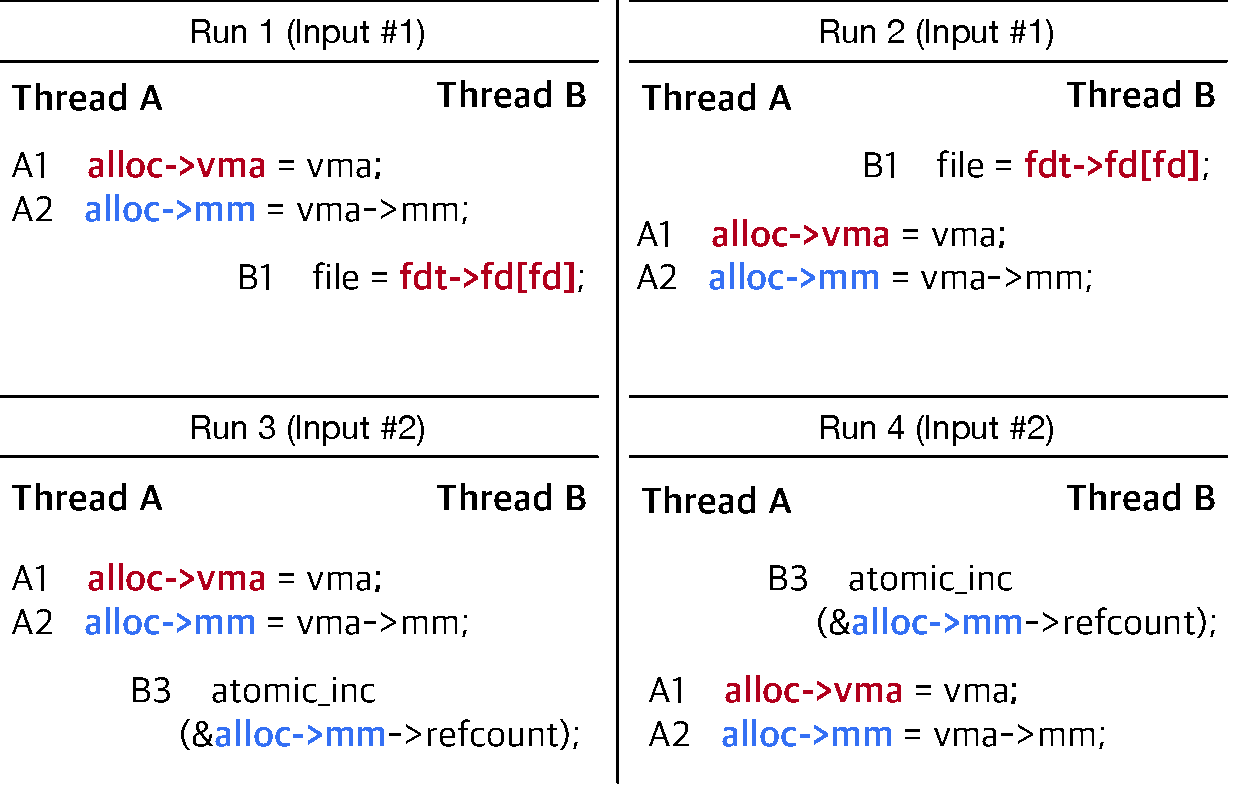
\includegraphics[width=0.9\linewidth]{fig/alias-coverage-interleaving.pdf}
  \caption{Four interleavings of \texttt{Input 1} and \texttt{Input 2}
    in \autoref{fig:alias-coverage}. After executing these four
    interleavings, all possible execution orders of a single
    conflicting accesses are exhibited.\dr{Run 1 -> Interleaving 1?}}
  \label{fig:alias-coverage-interleaving}
\end{figure}

In this example, if we adopt a coverage metric that focuses on a
single pair of conflicting accesses (\eg, alias coverage), a fuzzer
may not recognize that \texttt{Input 3} may exhibit a behavior
different than \texttt{Input 1} and \texttt{Input 2}~(\ie, a
NULL-dereference bug).
%
\autoref{fig:alias-coverage-interleaving} shows four interleavings
that exhibits all execution order of a single pair of conflicting
accesses. If a fuzzer executes \texttt{Input 1} with interleavings in
\texttt{Run 1} and \texttt{Run 2}, a fuzzer observes execution orders
such as $\texttt{A1} \rightarrow \texttt{B1}$ (in \texttt{Run 1}) and
$\texttt{B1} \rightarrow \texttt{A1}$ (in \texttt{Run 2}).
%
Similary, if a fuzzer executes \texttt{Input 2} with interleavings in
\texttt{Run 3} and \texttt{Run 4}, it observes execution orders of
$\texttt{A2} \rightarrow \texttt{B4}$ (in \texttt{Run 3}) and
$\texttt{B4} \rightarrow \texttt{A2}$ (in \texttt{Run 4}).
%
After executing these four interleavings, \texttt{Input 3} does not
reveal a new execution order of a single conflicting
accesses. Therfore, as a Krace state, a fuzzer may de-prioritize
\texttt{Input 3}, and the race condition may not be found.

In summary, in order to determine whether an input shows interesting
behaviors or not, a fuzzer needs to comprehend \textit{a combined
  result of multiple pairs of conflicting accesses} as it is the
primary reason of race conditions.


\cut{
Approaches that adopt a randomized scheduler~\cite{krace, ski, muzz}
suffer from the inherent randomness.
%
When the randomness comes to concurrency bugs, this could become a
significant drawback.
%
Although interleavings are affected by a fuzzer, a fuzzer cannot fully
control how interleaving takes place. Thus, a fuzzer may need to
indiscriminately execute the same input until its coverage is
saturated.
%
Furthermore, it is almost impossible for randomized schedulers to
expose concurrency bugs requiring an extreme interleaving such that
\dr{TODO: explain:}non-inclusive race conditions~\cite{exprace} or ones that
require a very small race window.
%
In contrast, approaches with a hint-directed scheduler is able to
explore all interelavings including even ones that hardly occur if a
proper scheduling hint is given. Therfore, they are able to find out
such race conditions.
%
However, existing approaches~\cite{razzer, snowboard} are not suitable
of diversifying interleavings. \ie, they change very small part of
interleaving across runs.
%
Even with a single input, they require a large number of execution to
test the input enough.
}

\PP{Our goal}
%
Our goal is to design a fuzzer to effectively explore the interleaving
space with a purpose of testing combinations of multiple pairs of
conflicting accesses as many as possible.
%
% Considering characteristics of concurrency bugs mentioned above, it
% will increase the probabilty of finding more concurrency bugs if we
% diversify interleavings to experience such partial orders as many as
% possible.
%
To this end, we organize subgoals as follows:
%
1) We first design a coverage metric to track combinations of pairs of
conflicting accesses,
% By this coverage metric, we do not waste the
% computing power for uninteresting inputs, and not de-prioritize inputs
% in which there are more unexplored interleavings.
%
2) based on the coverage metric, we design an interleaving mutation
mechanism that quickly saturate the coverage metric, and lastly,
%
3) we combine the coverage metric and the interleaving mutation
mechanism into Syzkaller~\cite{syzkaller} to find out race conditions
in the Linux kernel.



%
% This scheduling mechanism not only makes the investigation of such
% partial orders faster, but also does not miss concurrency bugs caused
% by an ``extreme'' interleaving (\ie, ones that hardly occur with the
% kernel scheduler).
% %
% % - observe an outcome
% %   - not to miss race conditions
% 3) While scheduling instructions, we detect concurrency bugs through
% abnormal behaviors instead of relying on data race detectors.
% %
% Although data race detectors are useful development tools, they are
% inherently limited in detecting race conditions.
% %
% We thus choose to observe the direct evidence of manifestation of
% concurrency bugs, an abnormal behavior.
% %
% Incorporating a data race detector will be discussed in
% \autoref{s:discussion}.



%%% Local Variables:
%%% mode: latex
%%% TeX-master: "p"
%%% End:

\section{Motivation}
\label{s:motivation}
\yj{Revise hint: Flow-OK, Clarification of text-Need work}

% - characteristics of concurrency bugs
% - challenges / design requirements
% - limitations of existing approaches


\dr{Not-defined terms: interleaving order, instance of thread
  interleaving ( = interleaving instance), multi-thread input}


\dr{TODO: muzz, conzzer}
%
This work is motivated by an observation that none of previous works
properly addresses characteristics of \textit{offending thread
  interleaving} (\ie, one that causes a concurrency bug).
%
As a consequence, previous works either \textbf{1)} suffer from
identifying whether offending thread interleaving remains
untested~\cite{krace}, or \textbf{2)} waste the computing power by
ineffectively exploring the search space of thread
interleaving~\cite{snowboard, razzer}.


In this section, we first comprehend why concurrency bugs manifest
depending on thread interleaving through a real-world concurrency bug
example.
%
We then define design goals to effectively discover concurrency bugs
in the kernel, and summarize why existing approaches fall short in
satisfying the design goals.


\PP{Manifestation of concurrency bugs}\yj{shorten this paragraph}
%
\begin{figure}[t]
  \centering
  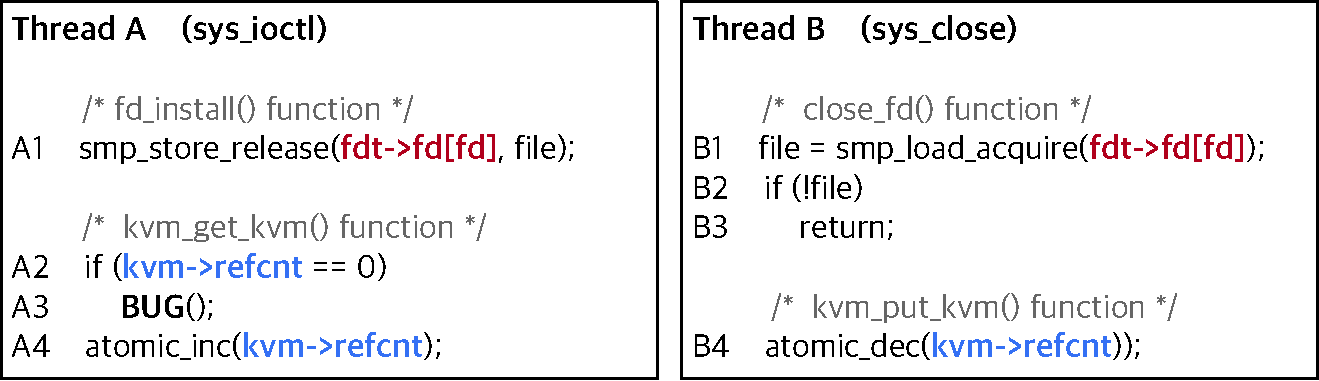
\includegraphics[width=0.95\linewidth]{fig/cve-2017-10661.pdf}
  \caption{Simplified code snippet of CVE-2017-17712. If \texttt{B1} is
    executed between \texttt{A2} and \texttt{A4}, a concurrency bug on
    \texttt{inet->hdrincl} leads to uninitialized stack pointer usage
    on \texttt{rfv}, and an attacker may gain root privileges.\yj{I do not know how attacker can gain a root privilege}}
  \label{fig:cve-2019-6974}
\end{figure}
%
\autoref{fig:cve-2019-6974} describes how an erroneous instance of
thread interleaving causes a concurrency bug.
%
In this example, an uninitialized access bug may manifest when two
system calls are executed concurrently: \texttt{sendmsg()} to send a
message through an ipv4 socket, and \texttt{setsockopt()} to modify an
option of the ipv4 socket. As a consequence of the uninitialized
access bug, an attacker may gain root privileges.



Assuming \texttt{inet->hdrincl} is initially \texttt{1}, the
concurrency bug manifests depending on the execution order of three
memory accesses, \texttt{A2} and \texttt{A4} in thread~A, and
\texttt{B1} and in thread~B.
%
During sending a message through the ipv4 socket, thread~A reads a
value of \texttt{inet->hdrincl} twice at \texttt{A2} and \texttt{A4}.
%
However, since these two read operations are not atomically executed,
thread~B may intervene in the middle of these two read operations.
%
In that case, if \texttt{B1} is executed between \texttt{A2} and
\texttt{A4}, thread~A reads different values of \texttt{inet->hdrincl}
at \texttt{A2} and \texttt{A4}, and dereference \texttt{rfv} without
initializing it.


\PP{Combined interleavings}
This example indicates that the manifestation of a concurrency bug
depends on the execution order of multiple memory
accesses. Specifically, a concurrency bug is \textit{a combined result
  of a few interleaving orders}, where each interleaving order is
established on a pair of memory access operations that access the same
memory object.
%
In this example, \texttt{rfv} is not initialized only if \texttt{A2}
is executed before \texttt{B1}. Thus, the uninitialized access
requires an interleaving order
$\texttt{A2} \Rightarrow \texttt{B1}$~\footnote{In this paper,
  $\texttt{X} \Rightarrow \texttt{Y}$ denotes that \texttt{X} is
  executed before \texttt{Y}}.
%
Similary, an interleaving order on \texttt{B1} and \texttt{A4} is also
required for the concurrency bug to manifest since thread~A
dereferences uninitialized \texttt{rfv} only if
$\texttt{B1} \Rightarrow \texttt{A4}$.
%
To sum up, among all possible instances of thread interleaving, only
ones that \textit{conjunctively satisfy the two interleaving orders,
  \ie,
  $(\texttt{A2} \Rightarrow \texttt{B1}) \wedge (\texttt{B1}
  \Rightarrow \texttt{A4})$}, can cause the concurrency bug while and
all other interleaving instances cannot.

\PP{Design goals}
%
The main goal of this paper is to design a fuzzing technique to
effectively discover kernel concurrency bugs. To this end, we identify
two design goals of a concurrency fuzzer as follows:

\vspace{0.4em}
\begin{enumerate}[label=\textbf{R\arabic*:}]
%
\item \emph{A fuzzer should be able to determine that offending thread
    interleaving remains untested.}
\item \emph{A fuzzer should be able to quickly trigger untested
    offending thread interleaving.}
%
\end{enumerate}

For example in \autoref{fig:cve-2019-6974}, \textbf{R1} states that a
fuzzer should adopt a proper interleaving coverage metric that can be
used to determine whether
$(\texttt{A2} \Rightarrow \texttt{B1}) \wedge (\texttt{B1} \Rightarrow
\texttt{A4})$ remains untested or not, and \textbf{R2} describes that
if this conjunctive condition has not been tested, a fuzzer needs to
schedule instructions to quickly cover the conjunctive condition
instead of exploring the entire search space of thread interleaving
randomly.

\dr{TODO: emphasize the size of thread interleaving space}

\subsection{Limitation of prior approaches}
\label{ss:existingapproaches}

Even though prior approaches achieve their own successes, none of them
satisfy \textbf{R1} and \textbf{R2}.

\PP{Insufficient coverage metric}
%
\begin{figure}[t]
  \centering
  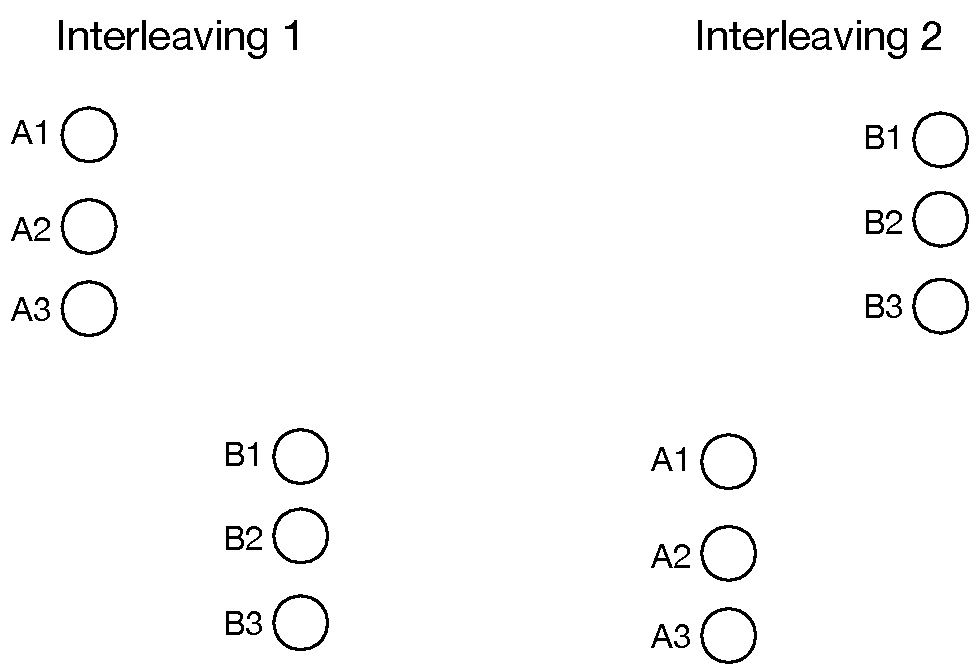
\includegraphics[width=0.95\linewidth]{fig/alias-coverage.pdf}
  \caption{Two instances of thread interleaving between thread~A and
    thread~B described in \autoref{fig:cve-2019-6974}. Regarding
    \texttt{inet->hdrincl}, alias coverage is saturated but the
    concurrency bug doest not manifest.}
  \label{fig:alias-coverage}
\end{figure}
%
To the best of our knowledge, existing concurrency coverage metrics
are not sufficient to determine whether interesting (\ie, offending)
thread interleaving remains untested. Thus, they do not satisfy
\textbf{R1}.
%
In particular, after KRace~\cite{krace} first emphasizes the necessity
of a coverage metric in the concurrency dimension, different
concurrency coverage metrics are proposed such as \textit{alias
  coverage}~\cite{krace}, \textit{concurrent call
  pair}~\cite{conzzer}, and \textit{\dr{TODO: MUZZ
    coverage}}~\cite{muzz}.
%
\yj{This paragraph must be easy enough for reader to intuitively understand, but hard to digest discussions}
However, they are not applicable to track behavioral changes\yj{what does it mean?} according
to a combination of interleaving orders, mainly because they either
track only a \textit{single} interleaving order~\cite{krace, muzz} or
\textit{coarse-grained information} such as a pair of two
concurrently-executed functions~\cite{conzzer}.
\yj{I do not understand why tracking a single int. order and coarse-grain information are not able to track behavioral changes}

Taking the example of KRace's alias coverage, \autoref{fig:alias-coverage}
describes two interleaving instances that saturate alias coverage
found between two system calls in \autoref{fig:cve-2019-6974}.
%
In these example interleaving scenarios, the uninitialized access does
not manifest even after alias coverage is saturated, and a fuzzer may
decide to stop searching for new interleaving instances in the two
system calls.
%
While we do not enumerate all proposed interleaving coverage metrics
here, we find that they all share the same limitation.


\PP{Ineffective scheduling mechanism}
%
Stemming from insufficient coverage metrics, proposed scheduling
mechanisms are also ineffective in satisfying \textbf{R2}.
%
As described in \autoref{s:background}, proposed scheduling mechanisms
are largely categorized into two: a randomized scheduler and a
hint-directed scheduler.

\dr{revisit after evaluation. not ready to write this part:}
%
Randomized schedulers~\cite{krace, pctalgorithm, muzz, ski} pay little
attention on collected interleaving coverage when scheduling
instructions, and rely on the randomness in diversifying thread
interleaving.
%
Therefore, they are inherently limited in satisfying a specific
condition of thread interleaving (\eg,
$(\texttt{A2} \Rightarrow \texttt{B1}) \wedge (\texttt{B1} \Rightarrow
\texttt{A4})$ in \autoref{fig:cve-2019-6974}).
%
This limitation is even more pronounced by a recent study,
ExpRace~\cite{exprace}, stating that many concurrency
bugs~\cite{cve20196974, cve20191999, cve201911486} manifest only if
thread interleaving satisfies an extreme condition that randomized
scheduler hardly satisfy.
%
Unfortunately, ExpRace demonstrates that this kind of concurrency bugs
are equally threatening the security of the kernel.


Whereas, % hint-directed schedulers~\cite{razzer, snowboard} enforce
% thread interleaving, and thus, are able to deterministically trigger
% concurrency bugs, even those that manifest under an extreme condition
% of thread interleaving.
% %
% However, 
state-of-the-art approaches adopting a hint-directed
scheduler, Razzer~\cite{razzer} and Snowboard~\cite{snowboard}, are
not capable of diversifying thread interleaving across iterations.
%
Since they do not adopt interleaving coverage, they are not able to
determine which thread interleaving requires further
testing. Therefore, they vary thread interleaving a small degree
across fuzzing iterations, and require a long time to trigger
concurrency bugs.
%
According to our evaluation~\autoref{s:eval}, ...


% In the perspective of fuzzing, a coverage metric is a paramount gear
% to determine whether a given input is worthy of further mutation.
% %
% If a coverage metric does not represent whether an input has a
% potential to trigger a race condition, a fuzzer may ignore inputs in
% which there are unexplored interleavings, or waste the computing power
% to valueless inputs.
% %
% In this regard, our primary question is whether existing coverage
% metrics in the concurrency dimension are suitable to apprehend
% interleavings potentially causing a race condition, for example,
% $(\texttt{A1} \Rightarrow \texttt{B1}) \wedge (\texttt{B4} \Rightarrow
% \texttt{A2})$ in \autoref{fig:cve-2019-6974}.



% Unfortunately, we observe that none of existing approaches incorporate
% a proper coverage metric for race conditions.
% %
% A few of existing approaches~\cite{snowboard, razzer} do not adopt a
% coverage in the concurrency dimension at all. Therefore, they do not
% make a decision as to whether a given input is worth further testing.
% %
% Other approaches~\cite{krace, muzz} adopt coverage metrics that are
% not suitable for race conditions as they do not consider a combined
% result of multiple pairs of conflicting accesses. As a consequence,
% race conditions may not be exposed even after the coverages are
% saturated.
% %
% % Consequently, existing approaches have difficulty in distinguishing a
% % given input has a potential to cause an interesting behavior, \ie,
% % a race condition.



% \yj{This is the key paragraph to point out the limitation of previous approaches, but very vague. Make specific claims of why Kraces' alias coverage is insufficient by giving an example.}
% %
% In order to show why comprehending multiple pairs of conflicting
% accesses is important, let us suppose we have three inputs that
% consists of two concurrent syscalls as described in
% \autoref{fig:alias-coverage}.
% %
% For all inputs, thread~A executes a \texttt{mmap()} syscall to map the
% binder driver to a user address space while thread~B handles different
% ioctl requests such that \texttt{ioctl(FREE_BUFFER)},
% \texttt{ioctl(REPLY)}, and \texttt{ioctl(TRANSACTION)} for
% \texttt{Input 1}, \texttt{Input 2}, and \texttt{Input 3} respectively.
% %
% It is worth noting that in \texttt{Input 1} and \texttt{Input 2},
% there is only one pair of conflicting accesses; in \texttt{Input 1},
% the two threads conflict on \texttt{alloc->vma}, and in \texttt{Input
%   2}, the two threads conflict on \texttt{alloc->mm}.



% \begin{figure}[t]
%   \centering
%   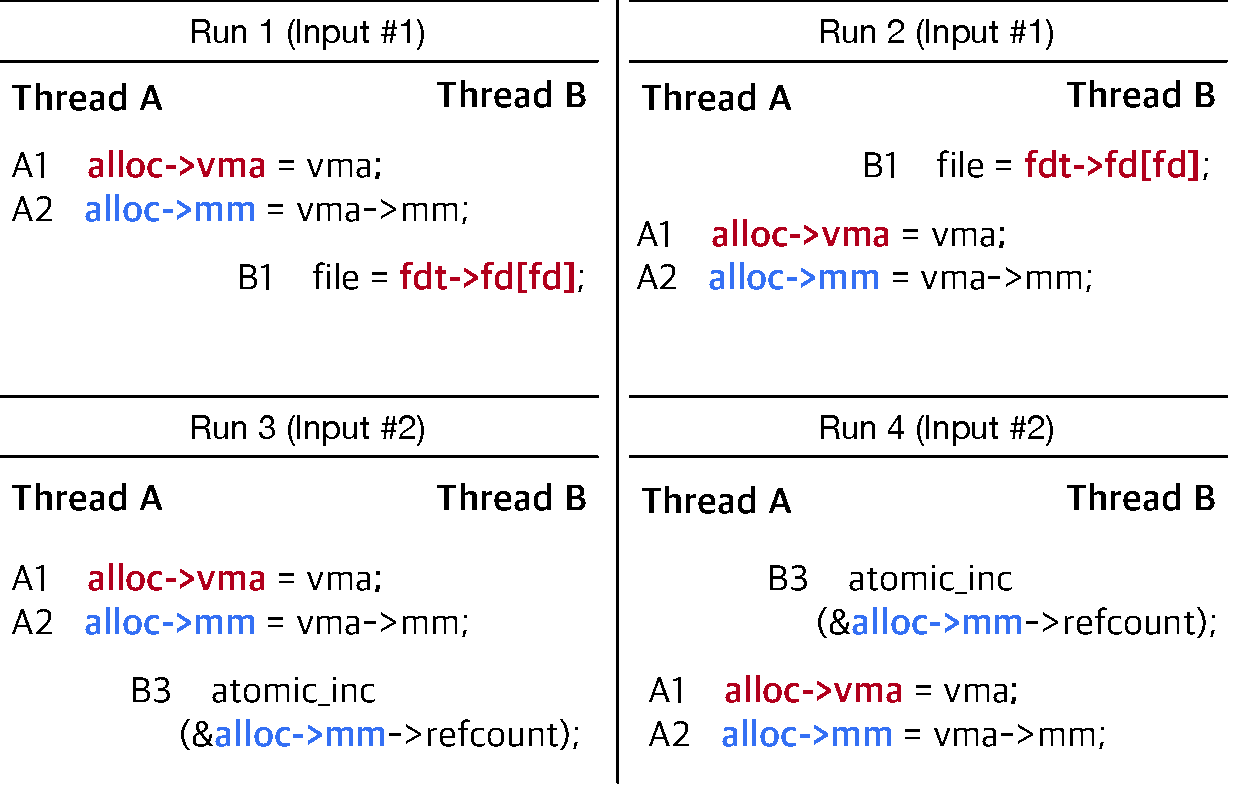
\includegraphics[width=0.9\linewidth]{fig/alias-coverage-interleaving.pdf}
%   \caption{Four interleavings of \texttt{Input 1} and \texttt{Input 2}
%     in \autoref{fig:alias-coverage}. After executing these four
%     interleavings, all possible execution orders of a single
%     conflicting accesses are exhibited.\dr{Run 1 -> Interleaving 1?}}
%   \label{fig:alias-coverage-interleaving}
% \end{figure}

% In this example, if we adopt a coverage metric that focuses on a
% single pair of conflicting accesses (\eg, alias coverage), a fuzzer
% may not recognize that \texttt{Input 3} may exhibit a different
% behavior than \texttt{Input 1} and \texttt{Input 2}~(\ie, a
% NULL-dereference bug).
% %
% \autoref{fig:alias-coverage-interleaving} shows four interleavings
% that exhibits all execution order of a single pair of conflicting
% accesses. If a fuzzer executes \texttt{Input 1} with interleavings in
% \texttt{Run 1} and \texttt{Run 2}, a fuzzer observes execution orders
% such as $\texttt{A1} \Rightarrow \texttt{B1}$ (in \texttt{Run 1}) and
% $\texttt{B1} \Rightarrow \texttt{A1}$ (in \texttt{Run 2}).
% %
% Similary, if a fuzzer executes \texttt{Input 2} with interleavings in
% \texttt{Run 3} and \texttt{Run 4}, it observes execution orders of
% $\texttt{A2} \Rightarrow \texttt{B4}$ (in \texttt{Run 3}) and
% $\texttt{B4} \Rightarrow \texttt{A2}$ (in \texttt{Run 4}).
% %
% After executing these four interleavings, \texttt{Input 3} does not
% reveal a new execution order of a single conflicting
% accesses. Therfore, as a Krace state, a fuzzer may de-prioritize
% \texttt{Input 3}, and the race condition may not be found.

% In summary, in order to determine whether an input shows interesting
% behaviors or not, a fuzzer needs to comprehend \textit{a combined
%   result of multiple pairs of conflicting accesses} as it is the
% primary reason of race conditions.



%%% Local Variables:
%%% mode: latex
%%% TeX-master: "p"
%%% End:

\section{Exploring Interleaving Space}
\label{s:design}

\newcommand{\segment}{segment graph\xspace}
\newcommand{\segments}{segment graphs\xspace}
\newcommand{\Segments}{Segment graphs\xspace}

\newcommand{\mutable}{mutable edge\xspace}
\newcommand{\mutables}{mutable edges\xspace}
\newcommand{\immutable}{immutable edge\xspace}
\newcommand{\immutables}{immutable edges\xspace}


The essence of a concurrency fuzzing relies on how to explore the
interleaving space.
%
In this section, we describe our approach to effectively explore the
interleaving space.
%
We first introduce the key idea of our
approach~(\autoref{ss:keyidea}), and then based on the key idea, we
propose a novel coverage concept in the concurrency
dimension~(\autoref{ss:coverage}) and an instruction scheduling
mechanism (\ie, interleaving mutation) to unveil undisclosed
coverage~(\autoref{ss:scheduler}).

\subsection{Key Idea}
\label{ss:keyidea}

\PP{Challenges}
%
Even though testing combinations of multiple conflicting accesses
provides a good bug-finding capability, one could argue that it may
require too many execution as the number of such combination is too
large.

\dr{wip.}


Our intuition comes from an observation that even a non-failing
interleaving bears hints on which interleavings require further
testing.
%
For example, if two consecutive load operations reading from a memory
location are followed by a store operation writing to the same
location, we can easily deduce that there might be a single-variable
atomicity violation.
%
If we run an interleaving generated by rearranging these operations,
we can identify whether the atomicity violation actually occurs or
not.
%
Our approach to explore the interleaving space realizes this
intuition.


\begin{figure*}[t]
  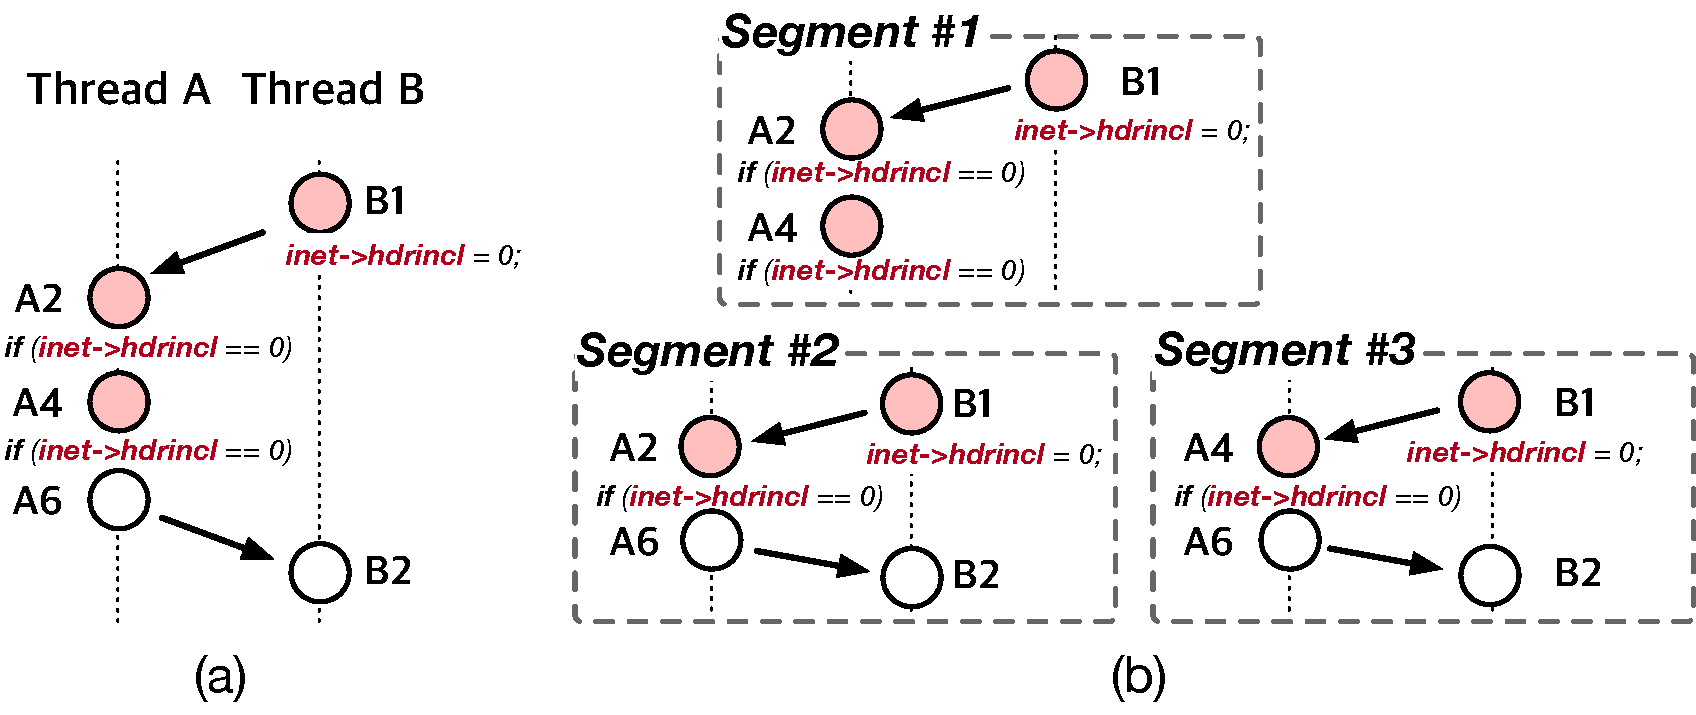
\includegraphics[width=0.9\linewidth]{fig/intuition.pdf}
  \caption{Key idea to explore the interleaving space. Each circle
    represents a memory access intruction. Annotations $R_x$ and $W_x$
    mean that the instruction reads from or writes to a memory
    location $x$ respectively.}
  \label{fig:intuition}
\end{figure*}


\PP{Overall steps}
%
Let us assume we obtain a totally ordered instruction sequence after
executing concurrent jobs~(\autoref{fig:intuition}-(a)).
%
In this instruction sequence, our purposes are 1) to track an
interesting behavior of the sequence, and 2) to schedule instructions
in the sequence for exposing more interesting behaviors.


As to tracking interesting behaviors, we follow the survey mentioned
in \autoref{ss:motivation} describing that most race conditions
deterministically manifest depending on a specific partial order of at
most four memory accesses.
%
According to this survey, such partial orders are ``interesting''
behaviors as they have a strong correlation to manifestation of
concurrency bugs.
%
Therefore, our purpose in tracking interesting behaviors in the
concurrency dimension turns into identifying how such partial orders
are established in the given sequence.
%
To this end, we enumerate small groups of a few (\eg, four) memory
accesses brought in the given instruction
sequence~(\autoref{fig:intuition}-(b)).
%
As the execution order of memory accesses in each group are already
determined, each group explains a part of the interleaving, therefore,
we call each group a segment of interleaving, or shortly a segment.
%
During fuzzing, we keep tracking segments as the signal of new
interelavings of concurrent jobs.





After collecting segments of concurrent jobs, we need to run the
concurrent jobs with different interleaving to observe different
segments.
%
Instead of blindly scheduling instructions, we deduce what partial
orders need to be explored in advance.
%
In other words, we hypothesize imaginary segments derived from
collected segments for further testing~(\autoref{fig:intuition}-(c)).
%
For example, by rearranging instructions of \texttt{Segment 1}, we
derive an imaginary segment called \texttt{Segment 1'} that are not
yet observed.
%
These imaginary segments will be used as scheduling hints; our
instruction scheduling mechanism will enforce imaginary segments
during further fuzzing runs.
%
It is worth noting that segments may be identical since the execution
order of not-conflicting instructions does not affect the outcome.
%
In this example, \texttt{Segment 1'} and \texttt{Segment 1''} are
identical and we consider they are redundant.

As a last step, we generate a hypothetical interleaving containing
these imaginary segments and run the interleaving to observe an
outcome~(\autoref{fig:intuition}-(d)).
%
Among all imaginary segments, some of them can be enforced together,
while some cannot.  For example, \texttt{Segment 1'} and
\texttt{Segment 2'} may be enforced together as they do not make a
conflict on the execution order of instructions.
%
We call two imaginary segments are harmonious if they are able to be
enforced together.
%
As all imaginary segments are not harmonious to all others, we need to
run different interleavings multiple times. For each fuzzing run, we
repeat generating a hypothetical interleaving by gathering harmonious
segments until we consume all imaginary segments.

\PP{Interleaving in a graph form}
%
Our interleaving exploration mechanism requires a few operations on an
interleaving such as 1) rearranging instructions in a segment, 2)
gathering harmonious segments, and 3) generating a whole interleaving
carrying multiple segments.
%
We notice that if we consider an interleaving as a graph of partial
orders, all above operations become simple graph operations.

From a given interleaving, we draw a graph consisting of vertices
representing memory access operations and edges representing the
execution order of the operations that may change the outcome if
reversed.
%
\dr{explain more intuition:}
With this graph, the required operations are simplified as follows: 1)
rearranging instructions is done by changing the direction of edges,
2) we can determine segments are harmonious if there is no loop in a
graph, and 3) a topological sort on a grpah generates a whole
interleaving.


In the rest of this section, we define the graph form of an
interleaving, and then provide details of the interleaving mutation.


% Dealing with an instruction sequence in this perspective has the
% following advantages:
% %
% First, it reduces the complexity of the interleaving space from
% exponential to polynomial to the number of instructions.
% %
% It is well known that the number of possible interleaving
% exponentially grows to the length of an instruction
% sequence~\cite{sctbench}. The intractable number of possible
% interleavings has been known as the paramount challenge for finding
% race conditions.
% %
% However, if we restrict our focus on a small number (\eg, four) of
% instructions, testing possible orders of small segments becomes a
% tractable problem with a polynomial complexity.
% %
% Second, given a concurrent jobs, it is able to know whether the
% concurrent jobs are worth further testing.
% %
% Because of the nondeterministic nature of race conditions, some race
% conditions hardly manifests even after a long period of
% testing~\cite{exprace}.
% %
% Without a proper metric, a fuzzer is forced to choose to repeatedly
% test a single input that does not causes a race condition, or to throw
% away an input that actually causes race condition when a very specific
% condition is satisfied.
% %
% Lastly, we can infer which segments are tested and which are not.
% %
% As mentioned before, some race conditions hardly manifests. These race
% conditions requires a very small race window sized for a few assembly
% instructions~\cite{afpacket}, or a thread stalling for a long
% time~\cite{noninclusive1, noninclusive2}. Although the probability of
% hitting the condition of them is not zero, without directing an
% interleaving, a fuzzer likely wastes a computing power until the
% condition is met.
% %
% Knowing which segments are not tested can significantly help for these
% cases. With a help of a scheduling hint-drected scheduler, we can
% force execution to experience segments that are not yet tested.



\subsection{Interleaving Graph}
\label{ss:coverage}

\begin{figure}[t]
  \caption{interleaving graph}
  \label{fig:interleaving-graph}
\end{figure}

In order to represent a partial order of memory accesses, we propose a
form of directed acyclic graph (DAG) called interleaving graph.
%
An interleaving graph describes an interleaving of concurrent jobs,
and represents partial orders between instructions.
%
In an interleaving graph, vertices indicate memory access operations,
and edges represent partial orders between these operations.
%
If there is a path from a vertex from another vertex, then the
execution order of two operations is established.

We categorize edges into two types, called \immutables and \mutables.
%
A \immutable corresponds to a program order in which instructions
appear on a thread~\cite{frightening, lkmm}. As a program order is
defined between instructions executed by the same thread, all
\immutables connect instructions from the same thread.
%
On the other hand, a \mutable is responsible to connect conflicting
instructions that 1) are executed by different threads, 2) access the
same memory location, and 3) at least one of them is write.
%
Therefore, the execution order of instructions connected by a \mutable
may directly affect the behavior of a program.


\autoref{fig:interleaving-graph} shows an example of an interleaving
graph.
%
\dr{TODO:}


\dr{TODO: imprecise description}
%
In terms of interleaving, \immutables and \mutables have different
properties. Let us suppose we have two interleaving graphs derived
from different interleavings of the same concurrent jobs.
%
As \immutables represent program orders, direction of \immutables does
not differ in the two interleaving graphs.
%
Whereas, a direction of \mutables may be different in the two
interleaving graphs.
%
It is worth noting that an edge may appear in only one interleaving
graph regardless of its type. This is because the control flow may be
changed according to the change of the data flow.


\PP{Segment of interleaving graph as coverage}
%
Although all execution order of conflicting instructions (\ie,
\mutables) in an interleaving graph may affect an outcome, we
concentrate on a small number of instructions because a few
instructions are enough to cause most ``interesting'' behaviors, \ie,
race conditions.

\dr{divide?}
%
We thus divide the interleaving graph into a set of subgraphs called
interleaving segment graphs, short for \segments.
%
While the interleaving graph represents a whole interleaving, an
\segment is a subgraph of the given interleaving graph that contains
two \mutables and at most four vertices. In addition, vertices in a
\segment are connected by at least one \mutable.

We capture \segments as coverage of a given interleaving of concurrent
jobs.
%
If a new \segment is not found while continuing to run the concurrent
jobs with different interleavings, the concurrent jobs unlikely expose
a race condition. In other words, if we collect all \segments of
concurrent jobs, we can lower the priority of the concurrent jobs.
%
It is worth noting that we select four as the maximum number of
vertices in a \segment because not only it is enough for most race
conditions, but also \dr{}...

In order to identify \segments from execution, we need to know the
total order of memory accesses. Otherwise, we may miss the execution
order between instructions so cannot faithfully capture \segments.
%
Therefore, our scheduling mechanism serializes execution of concurrent
jobs during fuzzing. Details are described later in \autoref{s:impl}.


\subsection{Interleaving Mutation}
\label{ss:scheduler}

% Since concurrent jobs may reveal different behaviors depending on an
% interleaving, a concurrency fuzzer adopt additional mutation strategy
% called interleaving mutation.

Our interleaving mutation is designed in a different way from previous
studies.
% 
Instead of randomly selecting scheduling points~\cite{krace, ski} or
changing the execution order of a few instructions~\cite{razzer,
  snowboard}, we draw a whole hypothetical interleaving directed
towards uncaptured \segments.
%
To this end, our interleaving mutation consists of three steps:
%
1) identifying uncaptured \segments, 2) selecting \textit{harmonious}
\segments, and 3) generating scheduling points to test the selected
\segments.

\PP{Identifying uncaptured segment graphs}
%
Given \segments derived from an interleaving, identifying uncaptured
\segments is the first step of interleaving mutation for generating
another interleaving.
%
For each \segment, we change directions of \mutables to infer
uncaptured \segments.
%
As each \segment contains two \mutables, at most four uncaptured
\segments are derived for one \segment.

\dr{TODO:}...






\PP{Selecting interleaving segments to direct}
%
Given all uncaptured \segments, it is unlikely that all \segments can
be tested at once.
%
Our approach is to find out a subset of \segments that are
\textit{harmonious}. \Segments are harmonious if they do not form a
cycle in an imaginary graph.


It may require heavy computation to identify the largest subset that
are all harmonious to each other.
%
Instead of finding the optimal solution, we choose to use a greedy
algorithm.
%
Especially, given uncaptured \segments extracted from an interleaving
graph, our interleaving mutation starts by selecting a random
\segment.
%
And then it iteratively selects a \segment while confirming that the
selected \segment is harmonious.
%
Determining a given \segment is harmonious is conducted by checking a
loop in an accumulated interleaving graph.

\dr{TODO: describe an algorithm to check a loop. }
Its time complexity is $O(V)$.


\PP{Generating scheduling points}
%
After selecting harmonious \segments, generating scheduling points can
be easily done by conducting a topological
sort~\cite{topologicalsort}.
%
Since an imaginary interleaving graph is acyclic, a topological sort
always returns a sequence of vertices (\ie, instructions) that does
not violate a program order.
%
It is well known that the time complexity of a topological sort is
$O(V+E)$. Considering that the graph is sparse, $E$ is a small value
so the time complexity can be asymptotically considered as $O(V)$.
%
In this sequence, scheduling points are just instructions that the
preemption should happen; \ie, the next instruction is executed by a
different thread.
%


\dr{TODO: what if scheduling points are missing}


%%% Local Variables:
%%% mode: latex
%%% TeX-master: "p"
%%% End:

\section{Design of \sys}
\label{s:impl}

\sys is a coverage-directed concurrency fuzzer to effectively discover
concurrency bugs.
%
The key improvement of \sys lies in adopting interleaving segment
coverage and the coverage-directed interleaving mutation algorithgm
described in \autoref{s:design}.
%
In the following of subsections, we describe design details of the
userspace fuzzer~(\autoref{ss:fuzzer}), the target kernel
instrumentation~(\autoref{ss:instrumentation}), the execution
engine~(\autoref{ss:engine}), and the implementation details of
\sys~(\autoref{ss:impl}).


\subsection{Userspace Fuzzer}
\label{ss:fuzzer}



\begin{figure}
  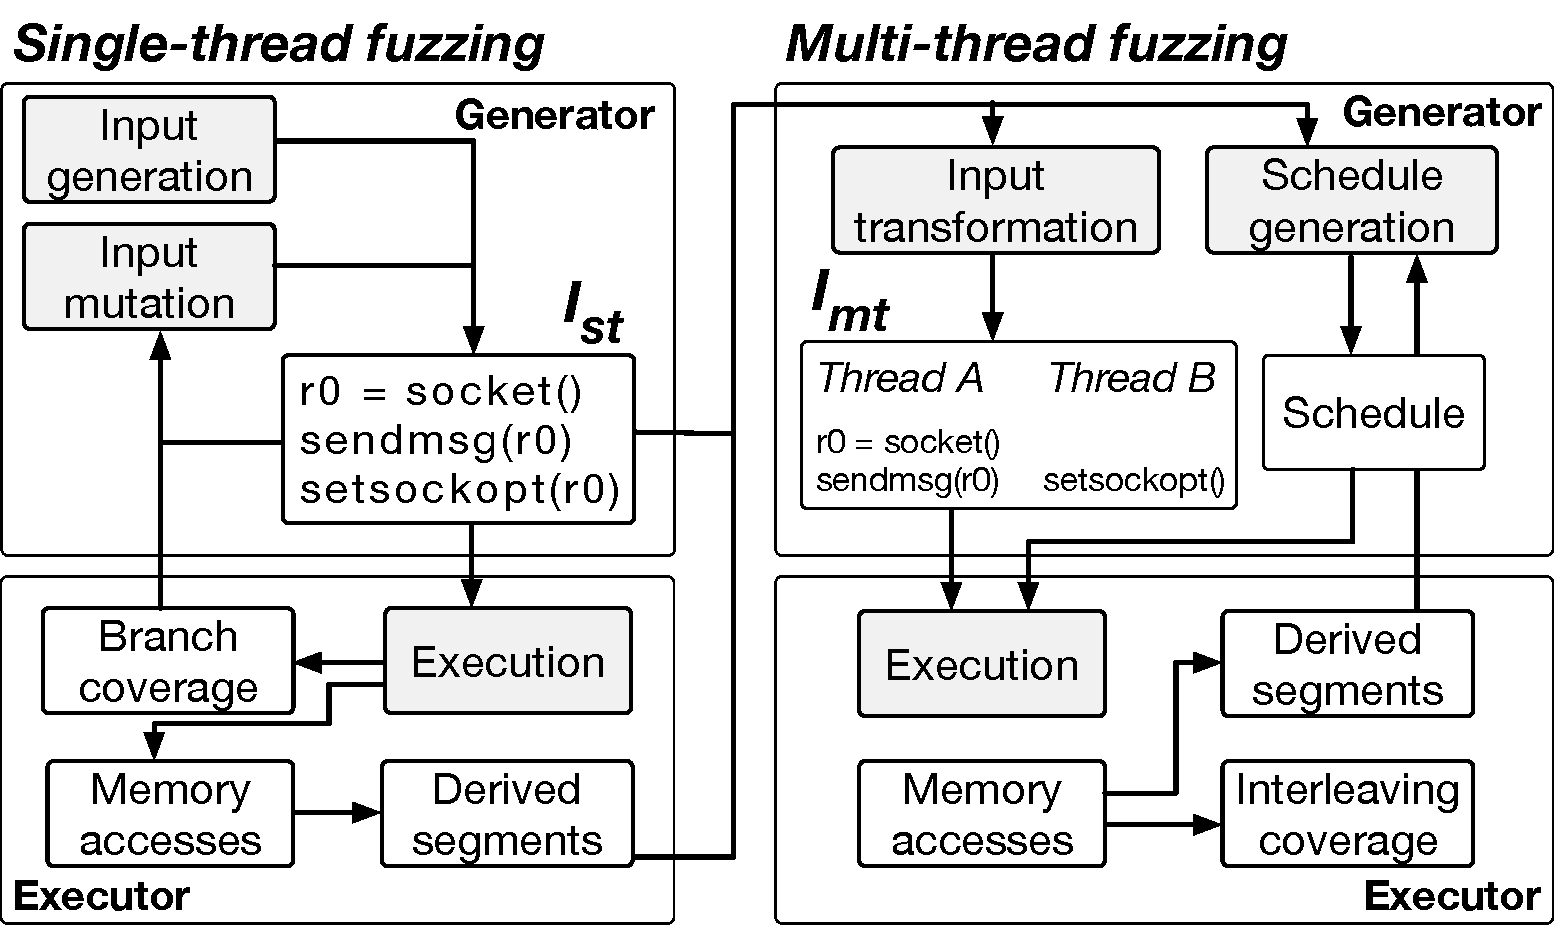
\includegraphics[width=0.9\linewidth]{fig/architecture.pdf}
  \caption{Workflow of \sys \dr{TODO: redraw to describe the workflow}}
  \label{fig:workflow}
\end{figure}


The \sys's userspace fuzzer conducts two-stage pipelined fuzzing
similar with recent concurrency fuzzers, Razzer~\cite{razzer} and
Snowboard~\cite{snowboard}.
%
In \sys, the first stage is a \textit{single-thread} fuzzing that
focuses on expanding code coverage, and the second stage is a
\textit{multi-thread} fuzzing to explore thread interleavings.

Both stages consists of two components, an input generator and an
input executor. We explain details of each component in the following.


\subsubsection{Single-thread fuzzing}
%
In a single-thread fuzzing phase, the single-thread generator
generates a single-thread input (refered as $I_{ST}$) in the form of a
sequence of random system calls.
%
And then, the single-thread executor executes $I_{ST}$ to perform two
things.
%
First, it collects code coverage of $I_{ST}$ with the purpose of
exploring source codes residing deep inside the kernel.
%
Second, it identifies two system calls in $I_{ST}$ that potentially
exhibit new interleaving coverage.  If identified, $I_{ST}$ will be
handed to the next phase, namely the multi-thread fuzzing.


\PP{Single-Thread Generator}
%
The single-thread generator is similar with conventional
fuzzing~\cite{syzkaller}.
%
It constructs a single-threaded system call sequence $I_{ST}$ with two
strategies: generation and mutation.
%
When using the generation strategy, \sys randomly generates a system
call sequence based on well-formed system call description grammar
\texttt{Syzlang}~\cite{syzlang}.
%
\texttt{Syzlang} describes templates of available system calls
including types of arguments and the type of a return value, as well
as a range of feasible values of each arguments.
%
According to \texttt{Syzlang}, \sys produces a single-thread system
call sequence by repeatedly selecting a random system call and
providing reasonable arguments of the system call.

The mutation strategy is an alternative of the generating strategy.
When using a mutation strategy, \sys picks up a already-generated
single-thread input, and modifies the single-thread input by appending
additional system calls, removing existing system calls, or changing
values of arguments of existing system calls.


\PP{Single-Thread Executor}
%
Given $I_{ST}$ from the single-thread generator, the single-thread
executor runs $I_{ST}$, and profiles basic blocks and memory accesses
executed by each system call with a support from instrumentation
detailed in \autoref{ss:instrumentation}.

With profiled basic blocks and memory accesses, the single-thread
executor conducts two tasks.
%
The first task is similar with what conventional kernel fuzzing
does.
%
In other words, the single-thread executor computes branch coverage
using profiled basic blocks.
%
Then, if $I_{ST}$ exposes new branch coverage that has not been
explored, \sys keeps $I_{ST}$, and feeds it back to the single-thread
generator so that the single-thread generator further mutates $I_{ST}$
to find more branch coverage.
%
As a result, \sys keeps a minimal set of $I_{ST}$, called a corpus,
which may execute previously-executed branches when running
single-thread inputs in the corpus.


Second, the single-thread executor identifies a pair of system calls
in $I_{ST}$ potentially exposes new interleaving coverage if executed
concurrently.
%
More specifically, for each pair of system calls, the single-thread
executor checks  \dr{}
%



\subsubsection{Multi-thread fuzzing}
%
After $I_{ST}$ is handed with a pair of system calls to execute
concurrently, the multi-thread generator transforms $I_{ST}$ to a
multi-thread input $I_{MT}$.
%
In addition, the multi-thread generator generates \textit{schedules}
where each schedule describes how to enforce thread interleaving (\ie,
a set of scheduling points) during runtime.


The multi-thread executor then repeatedly tests each schedule of
$I_{MT}$ one at at time.
%
To this end, the multi-thread executor instruments $I_{MT}$ with
hypercalls in order to tell the execution engine how to control thread
scheduling.
%
Lastly, the multi-thread executor runs $I_{MT}$ while enforcing a
given schedule with a support of the execution
engine~(\autoref{ss:engine}).




\PP{Multi-Thread Generator}
%
% In order to use interleaving graph as interleaving coverage, we need a
% method to store them, and compare them to a new interleaving graph.
% %
% We choose to use a hash value of

% the FNV-1~\cite{fnv, fnv-go}, non-cryptographic hash function,


% A schedule is an outcome of the interleaving mutation.
% A schedule contains an initial thread, and a set of scheduling points
% indicating an instruction on which preemption occurs.


\PP{Multi-Thread Executor}
%





\subsection{Target Kernel Instrumentation}
\label{ss:instrumentation}

\sys requires to profile basic blocks and memory accesses executed by
each system calls.
%
To this end, \sys incorporates a compiler pass that instruments
callbacks 1) at the beginning of each basic block, and 2) before each
instruction that access memory.
%
Each callbacks tracks basic blocks and memory accesses during the
execution in the kernel, records them into a shared memory regions.




% \autoref{fig:instrument} shows how the \sys's compiler pass transforms
% a binary.
% %
% During runtime, 


One important thing is that 




% Unlike data race detectors such as KCSAN~\cite{kcsan}, the \sys's
% scheduling mechanism needs to recognize both plane memory accesses and
% annotated memory accesses such as atomic operations.
% %
% We deal with these two types of accesses differently since annotated
% accesses usually are implemented in assembly code, which is hard for a
% LLVM pass to understand.
% %
% In order to instrument plane accesses, we implement a LLVM pass that
% insert callback function calls after memory accesses on LLVM IR.
% %
% Our pass runs after most of binary transfomration is done, so it
% \XXX{...}.
% %
% For annotated instructions, we rely on the functionality of
% KASAN~\cite{kasan} to instrument atomic operations.
% %
% KASAN provides wrapper functions of annotation APIs to call callback
% functions before annotated memory operations, and we instruct the
% wrapper functions to call our callbacks as well.
% %
% Our callbcak functions write memory access operations along with
% various information into a region mmap-ed shared region shared by a
% userspace program (\ie, fuzzer) and a kernel. The information about
% memory operations includes the instruction address, the start address
% of a memory location, and the size of memory access.
% %
% Accordingly, a fuzzer is able to identify what memory access
% operations took place during the execution.

% \sys also requires an additional module called a trampoline that is
% used to suspend and resume a running thread. Details about the
% trampoline are described in \autoref{ss:engine}.


\subsection{Execution Engine}
\label{ss:engine}

\begin{figure}
  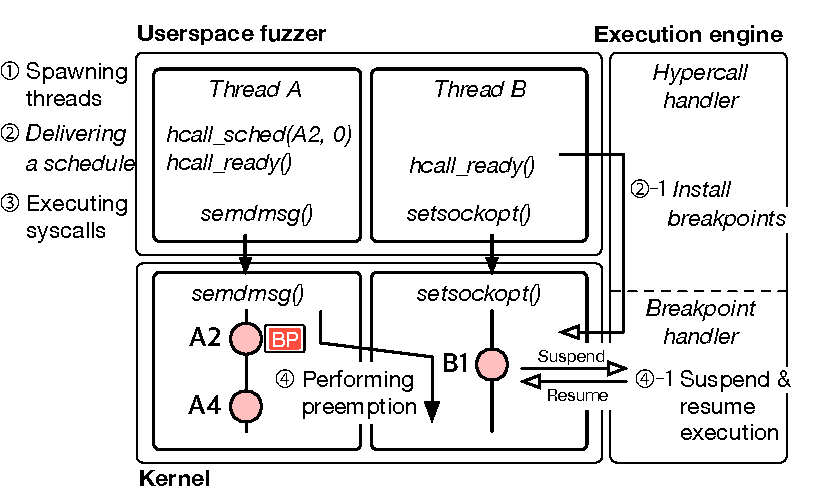
\includegraphics[width=0.9\linewidth]{fig/workflow-hypervisor.pdf}
  \caption{The workflow of the execution engine. \red{IMPORTANT: this
      is copied from AITIA. Need to redraw}}
  \label{fig:workflow-hypervisor}
\end{figure}

We introduce an execution engine in order to enforce an interelaving
provided by a fuzzer.
%
Specifically, the execution engine is to enforce an interleaving of
threads controlled by a fuzzer while all other kernel threads work
ordinarily.
%
During the execution, our hypervisor allows only one thread to execute
to make the execution serialized.
%
We implment the execution engine in the hypervisor layer to make it as
non-intrusive as possible.

\PP{Enforcing interleavings}
%
\autoref{fig:workflow-hypervisor} shows the overall workflow of our
execution engine.
%
The execution engine and a fuzzer communicates through hypercall
interfaces.
%
Scheduling points are sent from a fuzzer to the hypervisor before a
fuzzer executes concurrent syscalls.
%
\dr{TODO: how to send a schedule. what is a form of scheduling points}
A schedule is a specification of ...
%
After the fuzzer sends a schedule, the fuzzer notifies a hypervisor,
and the hypervisor starts executing with the intial thread specified
in the given schedule while other threads are suspended.
%
When the running thread reaches a scheduling point, a hypervisor
performs preemption by suspending the running thread and resuming the
next thread to run in order to enforce the execution order between
memory access operations.
%
\dr{TODO:}
Details about suspending and resuming a thread is described later.
%
\dr{TODO: how to handle missing breakpoints}


\PP{Suspending a thread}
%
A few prior approaches~\cite{ski, snowboard, razzer} suspend a vCPU
instead of a guest thread. While suspending a vCPU grants the ability
to control an interleaving, it is not suitable for our purpose because
suspending a vCPU may unexpectedly suspend another vCPU. An example we
observed is TLB shootdown~\cite{tlbshootdown}. When a vCPU wants TLB
shootdown, it sends inter-process interrupts (IPIs) to all cores and
wait until all cores to execute the TLB shootdown handler.  In this
case, if one vCPU is entirely suspended, the TLB shootdown cannot be
successfully conducted causing the vCPU invoking TLB shootdown
blocked.
%
Therefore, instead of adopting the prior approach, our hypervisor is
designed to suspends and resumes a guest thread.
%
In order to suspend a thread at an arbirary location, we use a
hardware breakpoint functionality~\cite{hwbp} shipped in modern Intel
CPU chipsets.
%
When a guest thread hits a breakpoint, our hypervisor saves its
register values and then changes the program counter of the thread to
an infinite loop called trampoline. In the trampoline, the thread
keeps calling \texttt{cond_resched()} to yield a CPU to make all other
kernel functionalities (\eg, handling the TLB shootdown handler) work
normally. When the guest thread resumes, our hypervisor restores
registers with the values saved when the thread is suspended, and the
thread continues its execution.


\PP{Virtual Machine Instrospection}
%
\dr{Not important contents but too long}
%
In the middle of execution, our hypervisor introspects the target
kernel for two reasons.
%
First, when a breakpoint is hit, it needs to determine whether the
breakpoint is hit by a fuzzer-controlled thread.
%
As a hardware breakpoint does not distinguish the running context of a
kernel, if the context switch happens, a breakpoint may be hit by
another thread or an interrupt handler, making the execution out of
expectation.
%
The hypervisor recognizes a running context using \texttt{task_struct}
which holds the thread description, and the per-cpu
\texttt{preempt_count} variable indicating what context the thread is
in (\eg, a task context for running a syscall, or a hardIRQ context to
handle hardware interrupts).
%
If a breakpoint is hit by a context other than the fuzzer-controlled
thread, our hypervisor ignores it and keeps the breakpoint.

Second, when a running thread tries to acquire a lock, our hypervisor
inspects the lock is held by a suspended thread.
%
When the suspended thread already acquires a lock while the running
thread wants to hold the same lock, the whole execution cannot make a
progress, because our hypervisor forces the lock-holding thread to
suspend.
%
Therefore, our hypervisor inspects whether the running thread is going
to be blocked due to the lock contention, and if it is, our hypervisor
takes control from the running thread to the suspended thread.
%
Inspecting the lock contention is conducted by hooking lockdep
functions~\cite{lockdep} that are commonly called from synchronization
prmitives.
%
When the lockdep functions are called, our hypervisor determins
whether the running thread can make a progress through various
information such as the address of the synchronization primitive, and
operation type (\ie, lock, unlock, and trylock).


\subsection{Implementation}
\label{ss:impl}

We implement \sys in various software layers.
%

%
To allow 


We use scc~\cite{scc} and sloccount~\cite{sloccount} to measure LoC of
GO and C respectively.


%%% Local Variables:
%%% mode: latex
%%% TeX-master: "p"
%%% End:

\section{Evaluation}
\label{s:eval}

To demonstrate the effectiveness of our approach, 
we evaluate \sys in various aspects.
%
Specifically, we 1) demonstrate the usefulness of \sys by providing
newly found concurrency bugs in the Linux
kernel~(\autoref{ss:realworldbugs}),
%
2) quantitatively compare \sys against prior concurrency fuzzing
techniques~(\autoref{ss:comparison}), and
%
3) analyze comprehensive performance characteristics of
\sys~(\autoref{ss:characteristics}).
%

\subsection{Finding Real-world Concurrency Bugs}
\label{ss:realworldbugs}

We run \sys to discover concurrency bugs in the latest Linux kernel.

\begin{table*}[t]
  \centering
  \resizebox{\linewidth}{!}{
  \begin{tabular}{r l l l l}
  \toprule
    Crash ID & Kernel Version (Commit) & Subsystem & Crash Type & Crash Summary \\
  \midrule
  1 \\
  \midrule
  2 \\ 
  \midrule
  3 \\
  \midrule
  4 \\
  \midrule
  5 \\
  \midrule
  6 \\
  \midrule
  7 \\
  \midrule
  8 \\
  \midrule
  9 \\
  \midrule
  10 \\
  \midrule
  11 \\
  \midrule
  12 \\
  \midrule
  13 \\
  \midrule
  14 \\
  \midrule
  15 \\
  \midrule
  16 \\
  \midrule
  17 \\
  \midrule
  18 \\
  \midrule
  19 \\
  \midrule
  20 \\
  \midrule
  21 \\
  \bottomrule
  \end{tabular}
}

%%% Local Variables:
%%% mode: latex
%%% TeX-master: "../p.tex"
%%% End:

  \caption{List of concurrency bugs newly discovered by \sys. The
    \texttt{Recurrent} column denotes that a crash was previously
    addressed but reoccurs even after its patch is applied.}
  \label{table:newbugs}
  \vspace{-5pt}
\end{table*}

\PP{Experimental setup.}
%
We run \sys on a two-socket machine equipped with
Intel(R) Xeon(R) CPU E5-2683 v4 @ 2.10GHz (40M cache) and 512\GB of
RAM.
%
This machine provides 32 total cores and 64 total threads, and runs
Ubuntu Server 20.04.4 LTS on Linux 5.4.143 as a host operating system.
%
During our experiments, we launch 32 virtual machines (VMs) where each
VM is equipped with four vCPUs and 8\GB memory.
%
We use a Linux kernel configuration used by
\texttt{Syzkaller}~\cite{syzkaller} so that \texttt{Syzkaller} and
\sys search the same kernel modules/subsystems.
The kernel versions we run on \sys ranges from 5.19-rc2 to 6.0-rc7.
%
%We run intermittently \sys for approximately two months on latest
%versions of the Linux kernel ranging from 5.19-rc2 to 6.0-rc7.


\PP{Newly found concurrency bugs.}
%
During our evaluation period, \sys discovers 83 unique crash titles including
ones that \texttt{Syzkaller} also finds. Among them, \totalbugs are
newly identified as harmful concurrency bugs. The result is summarized in
\autoref{table:newbugs}.
%
This table shows that \sys is able to find bugs across the entire
kernel layers from specific device drivers~(\eg, \texttt{\#1}, and
\texttt{\#6}) to various network subsystems (\eg, \texttt{\#2},
\texttt{\#16}, and \texttt{\#17}). 
Unlike KRACE, which focuses on 
kernel file systems, \sys is not tailored to specific subsystems.
%\sys entails the \textit{generality} and is
%applicable to various subsystems.
%
\sys is able to find not only less-harmful bugs such as warnings
(\eg, \texttt{\#12}) but also critical bugs such as memory corruptions
(\eg, \texttt{\#2}, \texttt{\#6}, and \texttt{\#14}).
%
It is worth noting that in our evaluation, all concurrency bugs are
found by observable and harmful incidents such as kernel panics or
KASAN reports.
%
Interestingly, we find that some bugs were previously found and
patched, but they reoccur in later kernel version because the patches are
incomplete fixes~\cite{learningfrommistakes}.
%
In \autoref{table:newbugs}, three that are marked in the
\texttt{Recurrent} column shows the cases that concurrency bugs reoccur.
%
These cases underline the significance of thorough testing even after 
bugs have been identified and supposedly fixed.

\subsection{Comparison with prior approaches}
\label{ss:comparison}

\begin{table}[t]
  \resizebox{\linewidth}{!}{
  \begin{tabular}{l l l l l}
    \toprule
    \textbf{Bug ID} & \textbf{Subsystem} & \textbf{Crash Type} & \textbf{Reference} \\
    \midrule
    CVE-2016-8655~\cite{cve20168655} & net/packet & use-after-free access & \cite{razzer, exprace} \\
    \midrule
    CVE-2017-2636~\cite{cve20172636} & drivers/tty & double-free & \cite{razzer, exprace} \\
    \midrule
    CVE-2017-7533~\cite{cve20177533} & fs/notify & slab-out-of-bound access & \cite{exprace} \\
    \midrule
    CVE-2017-17712~\cite{cve201717712} & net/ipv4 & uninitialized access & \cite{razzer, exprace} \\
    \midrule
    CVE-2019-1999~\cite{cve20191999} & drivers/android & double-free & \cite{exprace} \\
    \midrule
    CVE-2019-2025~\cite{cve20192025} & drivers/android & use-after-free access & \cite{exprace}  \\
    \midrule
    CVE-2019-6974~\cite{cve20196974} & virt/kvm & use-after-free access & \cite{exprace} \\
    \midrule
    CVE-2019-11486~\cite{cve201911486} & drivers/tty & use-after-free access & \cite{exprace} \\
    \midrule
    69e16d01d1de~\cite{snowboardbug} & net/l2tp & NULL dereference & \cite{snowboard} \\
    \bottomrule
  \end{tabular}
}

%%% Local Variables:
%%% mode: latex
%%% TeX-master: "../"
%%% End:

  \centering
  \caption{Known concurrency bugs that are studied in previous works,
    MoonShine~\cite{moonshine}, Razzer~\cite{razzer},
    ExpRace~\cite{exprace}, FUZE~\cite{fuze}, and
    Snowboard~\cite{snowboard}.}
  \label{table:knownbugs}
  \vspace{-5pt}
\end{table}

We compare \sys against prior approaches to answer the following
questions: 1) is interleaving segment
coverage~(\autoref{ss:coverage}) informative and helpful in
discovering concurrency bugs?  (\textbf{Design goal 1} in
\autoref{s:motivation})~(\autoref{sss:interleavingcoverage}), and
%
2) how is the mutation-based interleaving
exploration~(\autoref{ss:scheduler}) effective in exploring the search
space of thread interleavings? (\textbf{Design goal
  2})~(\autoref{sss:interleavingsearch}).
%
To evaluate the points, we collect well-known concurrency bugs as a test set, 
and then run \sys and prior approaches on the test set.

% 1) to demonstrate its
% performance improvement in discovering concurrency bugs
% (\autoref{sss:interleavingsearch}), and 2) justify the design choice
% of interleaivng segment coverage (\autoref{sss:interleavingcoverage}).

% interleaving segment coverage with alias coverage~\cite{krace} and
% concurrent call
% pair~\cite{conzzer}~(\autoref{sss:interleavingcoverage}).



\PP{Bug selection}
%
\autoref{table:knownbugs} shows concurrency bugs for the
comparison study.
%
Our concurrency bug selection criteria are 1)
concurrency bugs are used in previous studies~\cite{exprace, razzer,
  snowboard, moonshine, fuze}, and 2) their exploits are publicly
available so that we can make use of them for our evaluation.
%
However, there are few exceptions as follows: Although the exploit of
\texttt{69e16d01d1de}~\cite{snowboardbug} is not publicly available,
we successfully reproduce the concurrency bug from the description of
the Snowboard~\cite{snowboard} paper, so we include the bug.
%
% Whereas, even though Krace~\cite{krace} studies a subset of kernel
% concurrency bugs (\ie, data races), we do not take concurrency bugs
% from Krace, because we do not have access to ones used in Krace.
%
We exclude two Android-related concurrency bugs (\ie,
CVE-2019-1999~\cite{cve20191999} and CVE-2019-2025~\cite{cve20192025})
evaluated in ExpRace~\cite{exprace}.
%, because their exploits require to
%execute Android-specific code spaces where the current implementation
%of \sys (and \texttt{Syzkaller}) is limited to exploring.
To run tests on a consistent environment, we use the same kernel 
of version v6.0-rc7 and make the bugs available by rolling back patches 
that addressed concurrency bugs.

%\PP{Kernel preparation}
%
%Since concurrency bugs in \autoref{table:knownbugs} are introduced,
%found, and fixed at different times, it is hard to find a kernel
%version that is vulnerable to all listed bugs.
%
%Therefore, we inject the concurrency bugs into the Linux kernel
%version v6.0-rc7 by reverting patches fixing the concurrency bugs.



\PP{Comparison method}
%
We measure the number of executions and the elapsed time required to
discover each concurrency bug.
%
However, these metrics heavily depend on initial seeds and the process
of mutating multi-thread input seeds, which may vary across evaluations and 
disturb a fair fuzzing evaluation~\cite{fuzzingeval}.
%
To confine such noisy interference, we manually provide
a multi-thread input as well as a pair of system calls that triggers
each concurrency bug.
Therefore, we evenly compare how accurately and quickly fuzzers can discover 
concurrency bugs when bug-triggering inputs are given.
%
%Then, in all evaluations in this section, a fuzzer only explores
%thread interleavings of the multi-thread inputs we provide, without
%generating or mutating inputs.
%
%In this way, we do not need to consider the process of mutation, and
%can focus on the effectiveness of the thread interleaving exploration
%of each approach.
%
Also, during the evaluation, we limit the number of executions to
10000 for each measurement, which is large enough for our evaluation.
%
% \dr{I do not use the term ``random'' here because the thread
%   interleaving exploration is random anyway.}





\subsubsection{Comparison of interleaving coverage metrics}
\label{sss:interleavingcoverage}
%
In order to answer the question why a concurrency fuzzer should adopt an
informative interleaving coverage metric (\ie, interleaving segment
coverage), we demonstrate performance of \sys if it adopts a
less-informative interleaving coverage metric (\eg, alias
coverage~\cite{krace}).


\PP{Comparison target}
%
We choose alias coverage as a comparison target since it is an
interleaving coverage metric most relevant to interleaving segment
coverage (\ie, both describe interleavings of instructions).
%
However, alias coverage is implemented only for file systems, so we
emulate alias coverage in \sys by limiting the number of vertices of
each segment graph to two. Hence, like alias coverage,
interleaving segments of size 2 contains a single interleaving 
between two instructions where at least one of them is a write instruction.
%
Using the emulated alias coverage, we run \sys to see whether each
concurrency bug is triggered until the emulated alias coverage is
saturated.
% as a
% feedback of the \sys's speculative interleaving exploration, we run
% \sys with a fixed pair of system calls that can cause each concurrency
% bug, and measure two things: 1) the number of executions until each
% coverage metric is saturated, and 2) whether a given concurrency bug
% is triggered or not.


\PP{Result}
%
\begin{table}[t]
  \small
  \centering
  \resizebox{1\linewidth}{!}{
  \begin{tabular}{l l l l l l l l l l l l}
    \toprule
    \multirow{2}{*}{\textbf{Bug ID}} & \multicolumn{10}{c}{\textbf{Trials}} & \textbf{Avg.} \\
    & \textbf{\#0} & \textbf{\#1} & \textbf{\#2} & \textbf{\#3} & \textbf{\#4} & \textbf{\#5} & \textbf{\#6} & \textbf{\#7} & \textbf{\#8} & \textbf{\#9} & \textbf{exec.} \\
    \midrule
    CVE-2016-8655~\cite{cve20168655} & \checkmark & \checkmark & - & \checkmark & - & - & \checkmark & - & \checkmark & - & 9.4 \\
    % \midrule
    CVE-2017-2636~\cite{cve20172636} & - & -  & -  & -  & -  & -  & -  & -  & -  & -  & 8.4 \\
    % \midrule
    CVE-2017-7533~\cite{cve20177533} & - & -  & -  & -  & -  & -  & -  & -  & -  & -  & 32 \\
    % \midrule
    CVE-2017-17712~\cite{cve201717712} & -  & -  & -  & -  & -  & -  & -  & -  & -  & - & 21.5 \\
    % \midrule
    CVE-2017-15649~\cite{cve201715649} & \checkmark & - & \checkmark & \checkmark & \checkmark & - & \checkmark & \checkmark & \checkmark & - & 12 \\
    % \midrule
    CVE-2018-12232~\cite{cve201812232} & - & - & - & - & - & - & - & - & - & - & 16.0 \\
    % \midrule
    CVE-2019-6974~\cite{cve20196974} & - & - & - & - & - & - & - & - & - & - & 10.4 \\
    % \midrule
    CVE-2019-11486~\cite{cve201911486} & - & - & - & - & - & - & - & - & - & - & 6 \\
    % \midrule
    69e16d01d1de~\cite{snowboardbug} & \checkmark & \checkmark & \checkmark & - & \checkmark & \checkmark & \checkmark & \checkmark & \checkmark & \checkmark & 9.3 \\
    \bottomrule
  \end{tabular}
}

% Single
% cve-2016-8655 O
% cve-2017-15649 O
% cve-2017-17712 X
% cve-2017-2636 X
% cve-2017-7533 X
% cve-2018-12232 X
% cve-2019-6974 X
% cve-2019-11486 X
% 69e16d01d1d O



%%% Local Variables:
%%% mode: latex
%%% TeX-master: "../p"
%%% End:

  \caption{Trade-off between the bug-finding capability and the search
    complexity. Out of 10 trials using the less-informative
    interleaving coverage metric, \checkmark\xspace indicates that a
    bug is triggered, while - indicates that a bug is not
    triggered. The \texttt{Avg. exec.}  column denotes that the
    average number of execution until the saturation of interleaving
    coverage.}
  \label{table:aliascoverage}
  \vspace{-5pt}
\end{table}
%
\autoref{table:aliascoverage} shows the result.
%
When using emulated alias coverage, \textit{many (six ouf of nine)
concurrency bugs are not discovered even if emulated alias coverage
completely is saturated}.
%
The example of CVE-2017-17712 described in \autoref{s:motivation}
(\ie, \autoref{fig:cve-2017-17712}) explains why such poor results come 
out; alias coverage considers only interleavings between two
instructions, which is \textit{not sufficient} to execute the
offending interleaving containing multiple instructions. We manually 
identify that all
listed concurrency bugs are caused by thread interleavings of three or
four instructions, which supports our design choice on the size of
interleaving segments (\autoref{ss:overview}).
%
On the other hand, alias coverage is saturated quickly. With
our mutation-based interleaving exploration, it is saturated after 13.9
executions on average, ranging from 6 to 32.
%

\PP{Bug-finding capability and search complexity trade-off}
The result indicates the trade-off between the bug-finding
capability and the search complexity; Alias coverage shows the
\textit{lower} search complexity while it also shows the \textit{weaker}
bug-finding capability.
%
Whereas, using interleaving segment coverage, \sys can discover all listed
concurrency bugs before the saturation of interleaving
segment coverage. Thus, interleaving segment coverage shows the
\textit{stronger} bug-finding capability but it sets more larger search 
space than the alias coverage.
Hence, interleaving segment coverage entails the cost of the
higher search complexity. Nevertheless, we claim that 
its search complexity is still tractable to perform the mutation-based 
interleaving exploration, and we validate our claim  in the next
evaluation~(\autoref{sss:interleavingsearch}).


% that interleaving segment coverage is not saturated until a
% given concurrency bug is triggered (\ie, showing the strong
% bug-finding capability), while less-informative interleaving coverage
% (\eg, alias coverage) is saturated quickly (\ie, showing the low
% search complexity).




%
% As a consequence, we conclude that a fuzzer can rely on interleaving
% segment coverage when determining whether to stop probing new
% interleavings.




%






\subsubsection{Effectiveness of mutation-based interleaving
  exploration}
\label{sss:interleavingsearch}
%
% \begin{figure*}[t]
%   \centering
%   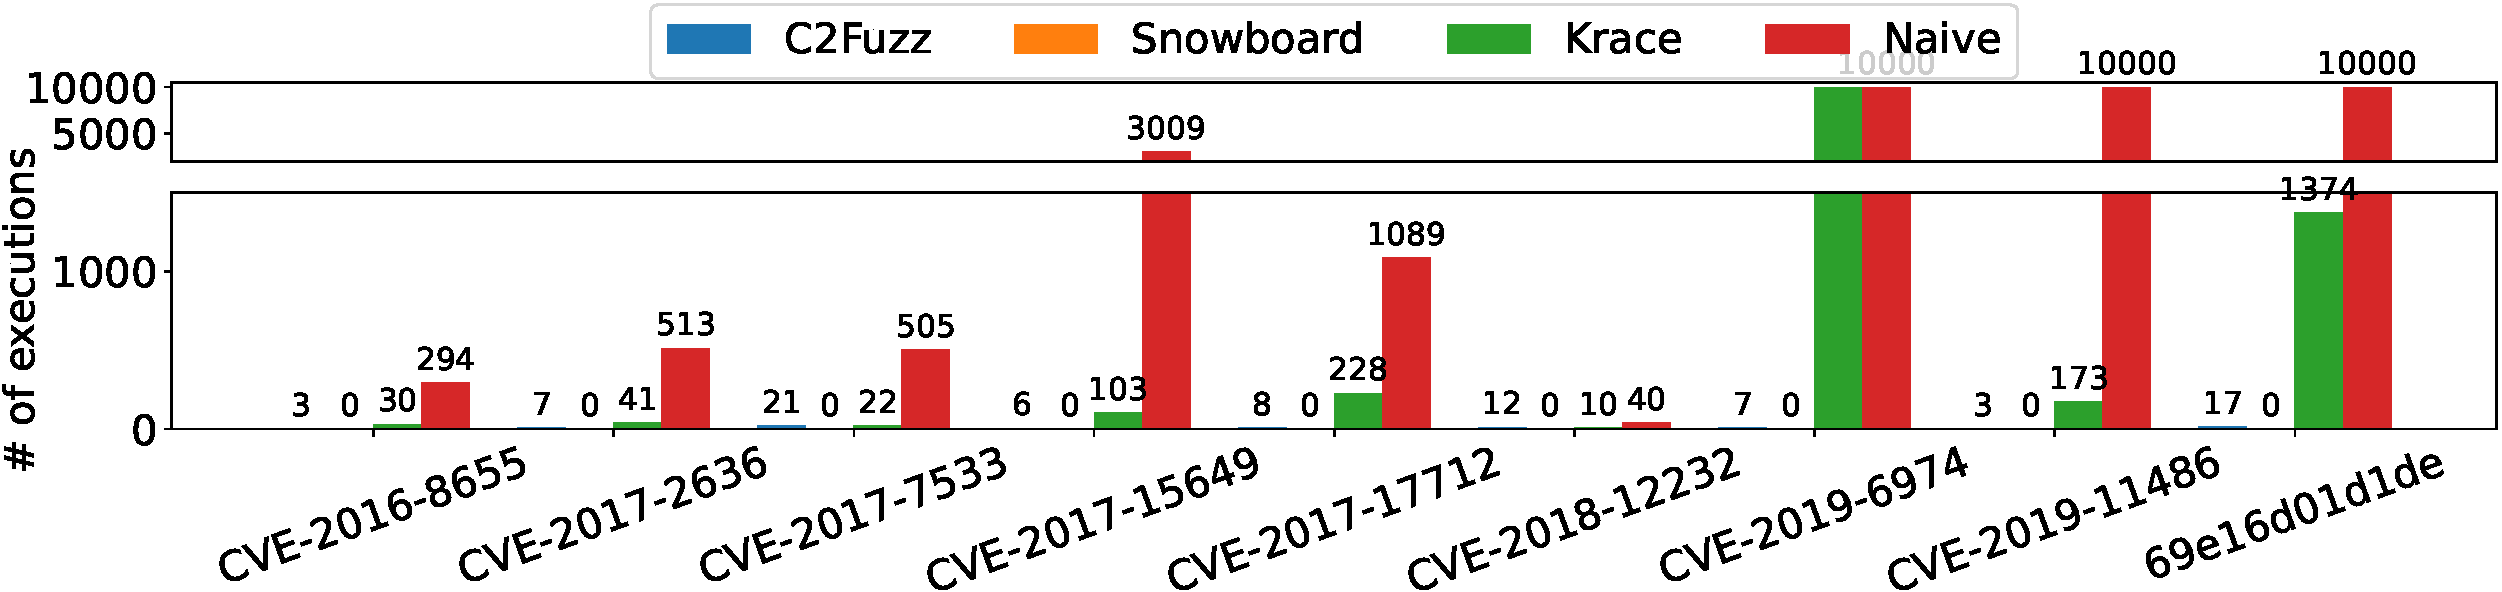
\includegraphics[width=\linewidth]{fig/comparison_graph-crop.pdf}
%   \caption{\dr{table is better?}}
%   \label{fig:eval:comparison}
% \end{figure*}
%
% \begin{table*}
%   \centering
%   \newcommand\mc[1]{\multicolumn{1}{l}{#1}}  % shortcut macro

\resizebox{0.9\linewidth}{!}{
  \begin{tabular}{l S[table-format=7.0] l S[table-format=7.0] l S[table-format=7.0] l S[table-format=7.0] l}
    \toprule
    \multirow{2}{*}{\textbf{Bug ID}} & \multicolumn{2}{c}{\textbf{\sys}} & \multicolumn{2}{c}{\textbf{Snowboard}~\cite{snowboard}} & \multicolumn{2}{c}{\textbf{Krace}~\cite{krace}} & \multicolumn{2}{c}{\textbf{Naive}} \\
    \cmidrule(rl){2-3} \cmidrule(rl){4-5} \cmidrule(rl){6-7} \cmidrule(rl){8-9}
    & \mc{\# of exec.} & Elapsed time & \mc{\# of exec.} & Elapsed time & \mc{\# of exec.} & Elapsed time & \mc{\# of exec.} & Elapsed time \\
    \midrule
    CVE-2016-8655~\cite{cve20168655} & 6 & 2.2 & 12 & 4.0 & 96 & 44.2 & 270 & 85 \\
    % \midrule
    CVE-2017-2636~\cite{cve20172636} & 22 & 7.1 & 58 & 26.4 & 9 & 4.4 & 721 & 377.8 \\
    % \midrule
    CVE-2017-7533~\cite{cve20177533} & 30 & 16 & 191 & 58 & 53 & 24.2 & 274 & 83.3 \\
    % \midrule
    CVE-2017-17712~\cite{cve201717712} & 17 & 5.4 & 79 & 22.2 & 1296 & 359.3 & 1757 & 474.2 \\
    % \midrule
    CVE-2017-15649~\cite{cve201715649} & 38 & 13.2 & 31 & 10.0 & 342 & 100.0 & 1852 & 460.8 \\
    % \midrule
    CVE-2018-12232~\cite{cve201812232} & 12 & 3.3 & 8 & 2.4 & 14 & 4.0 & 78 & 29.1 \\
    % \midrule
    CVE-2019-6974~\cite{cve20196974} & 81 & 52.4 & 229 & 139.4 & >10000 & >5720.1 & >10000 & >5578 \\
    % \midrule
    CVE-2019-11486~\cite{cve201911486} & 3 & <1 & 37 & 16.6 & 494 & 222.6 & >10000 & >3810 \\
    % \midrule
    69e16d01d1de~\cite{snowboardbug} & 41 & 23.2 & 156 & 61.8 & >10000 & >3410.5 & >10000 & >3358 \\
    \bottomrule
  \end{tabular}
}

%%% Local Variables:
%%% mode: latex
%%% TeX-master: "../p"
%%% End:

%   \caption{Result of the comparison study against various
%     state-of-the-art kernel concurrency fuzzers (\ie,
%     KRACE~\cite{krace} and Snowboard~\cite{snowboard}). We measure the
%     number of executions and the elapsed time (secs) required to
%     discover each concurrency bug. The \texttt{Naive} column indicates
%     the kernel's scheduler (\ie, no thread scheduling control applied).}
%   \label{table:comparison-interleaving-search}
%   \vspace{-5pt}
% \end{table*}

\begin{figure}[t]
  \centering
  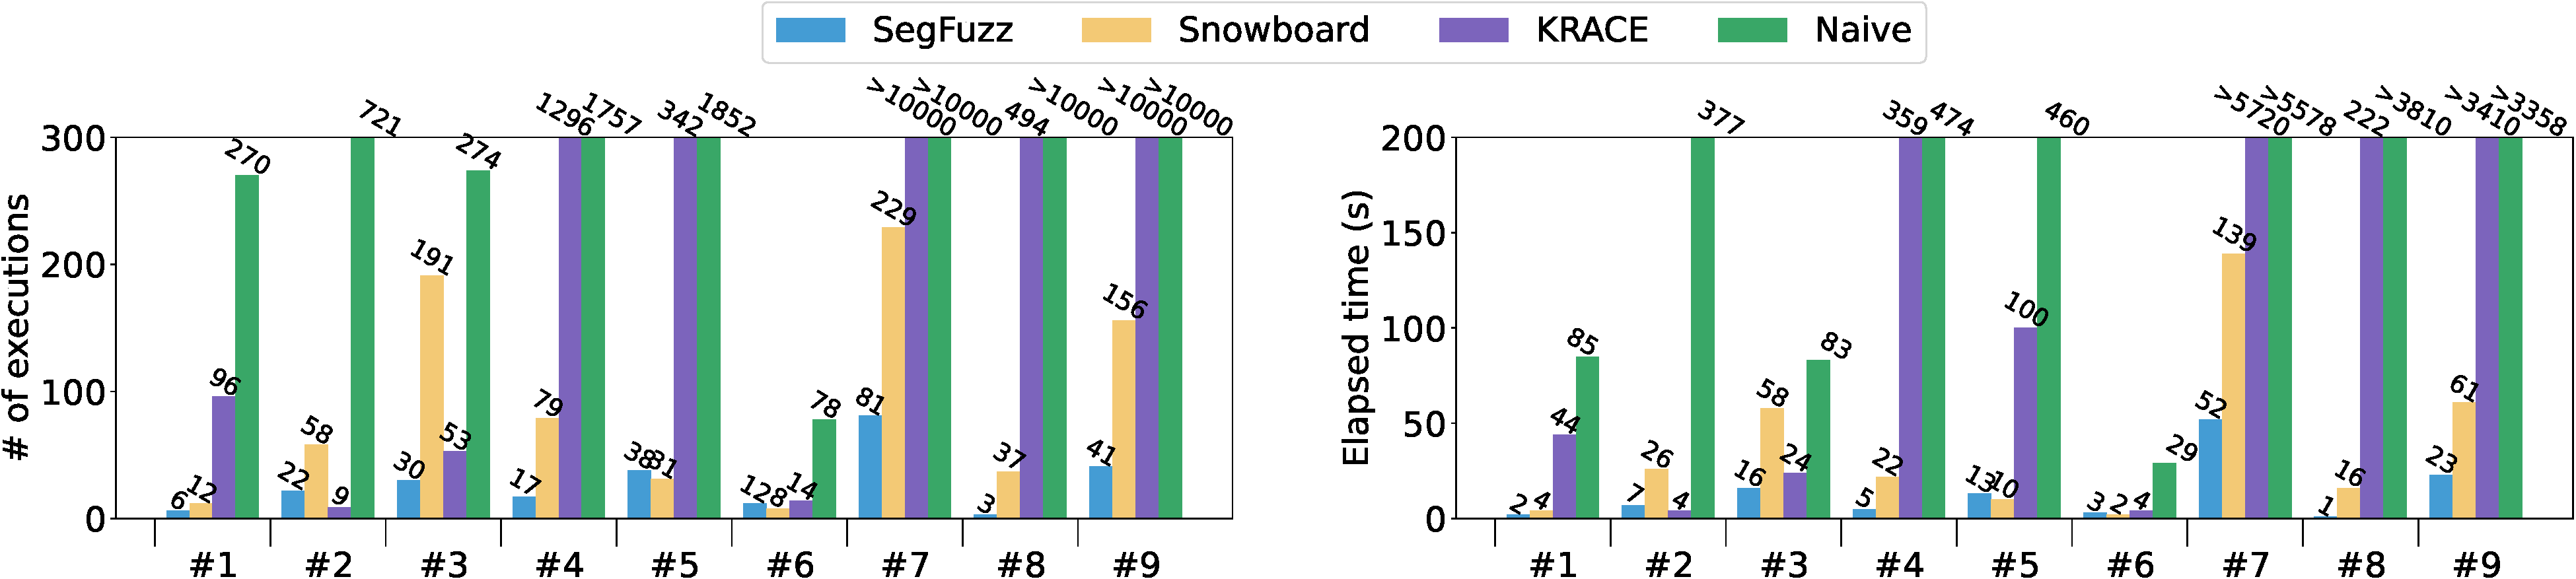
\includegraphics[width=0.99\linewidth]{fig/comparison_graph_execution-crop.pdf}
  \caption{Number of executions required for each concurrency fuzzer
    to discover concurrency bugs listed in
    \autoref{table:knownbugs}. The \texttt{Naive} column indicates the
    kernel's scheduler (\ie, no thread scheduling control applied).}
  \label{fig:eval:comparison-execution}
  \vspace{-8pt}
\end{figure}

\begin{figure}[t]
  \centering
  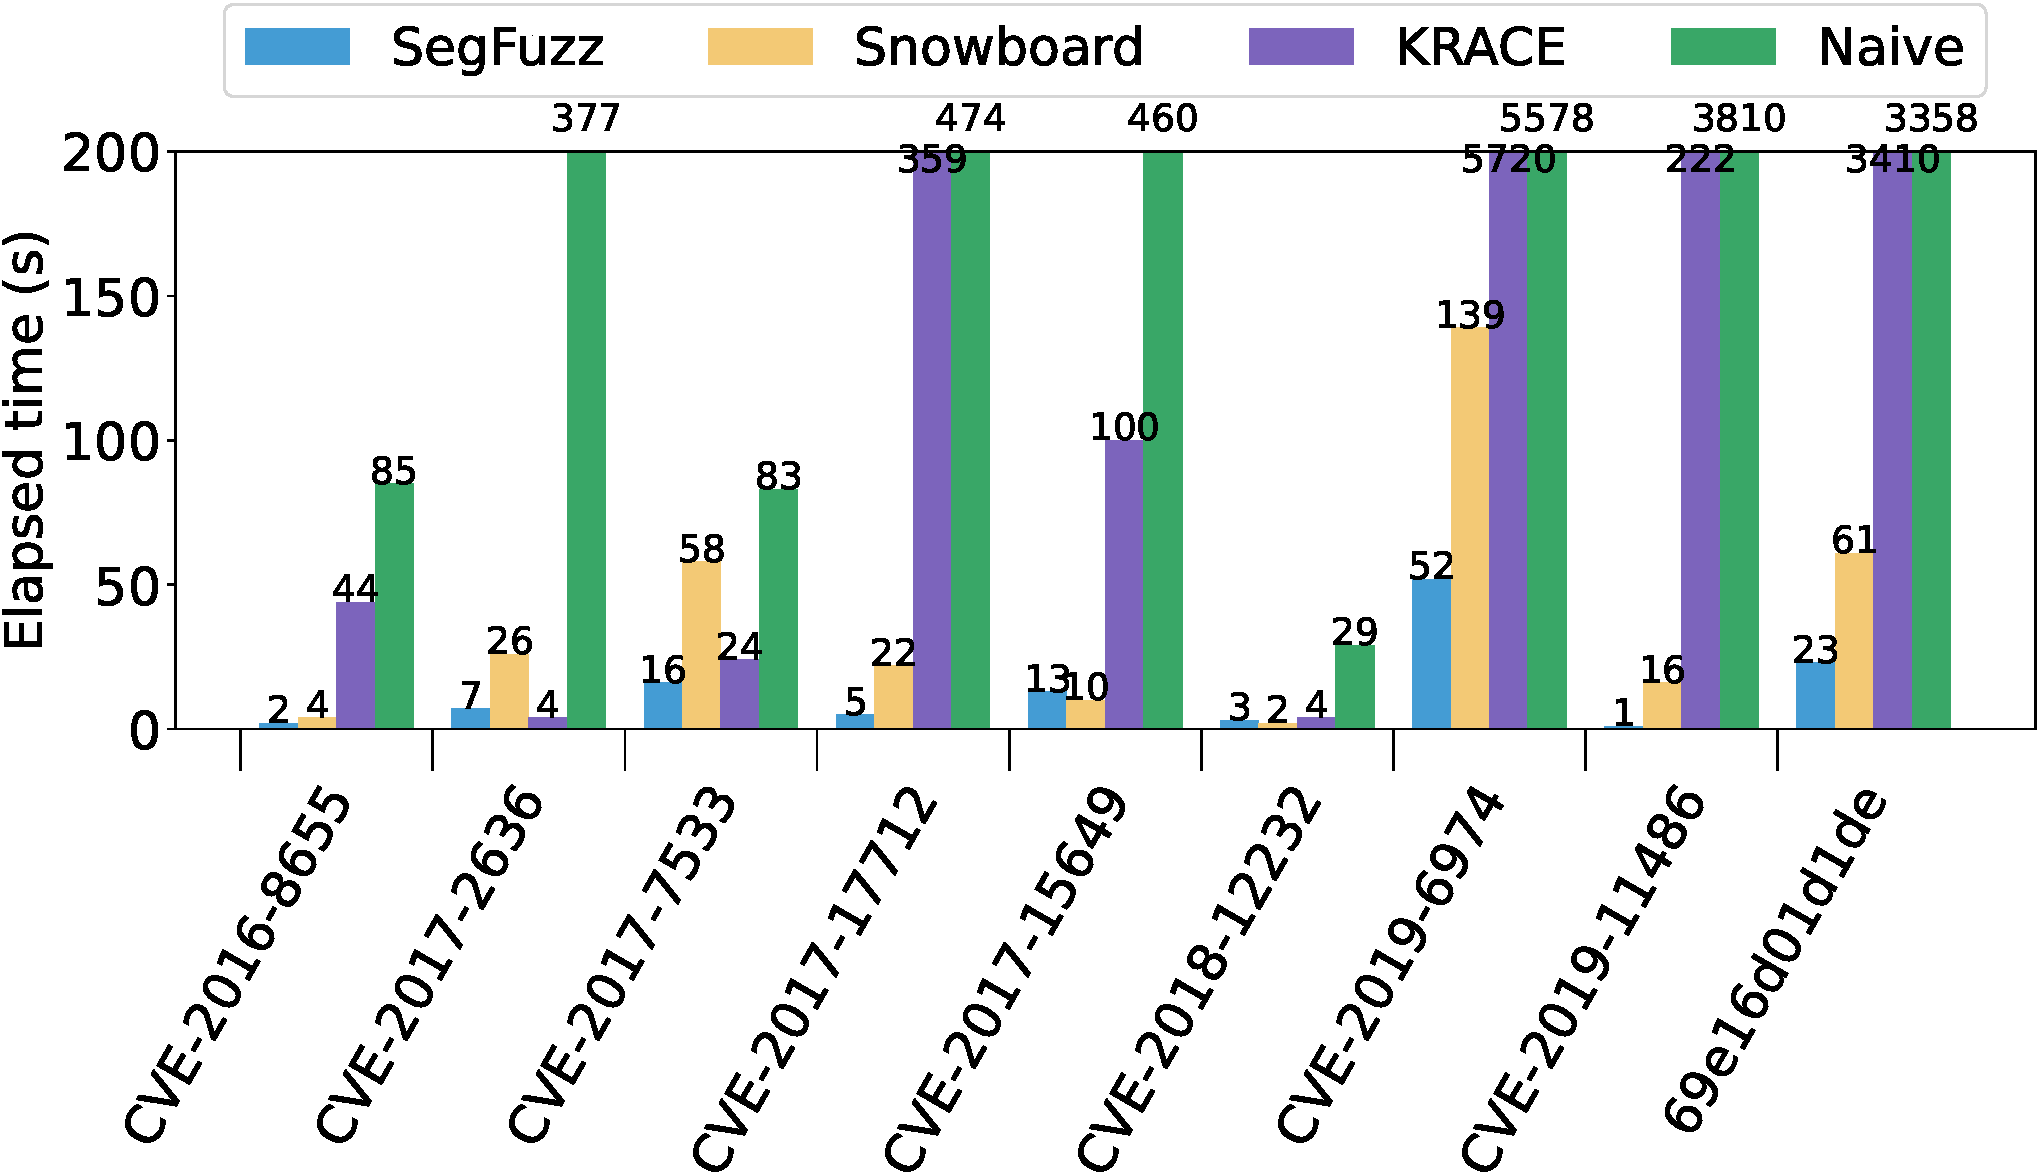
\includegraphics[width=0.99\linewidth]{fig/comparison_graph_time-crop.pdf}
  \caption{Elaped time required for each concurrency fuzzer to
    discover concurrency bugs listed in \autoref{table:knownbugs}.}
  \label{fig:eval:comparison-time}
  \vspace{-8pt}
\end{figure}

% \begin{figure*}
% \subfloat[First.]{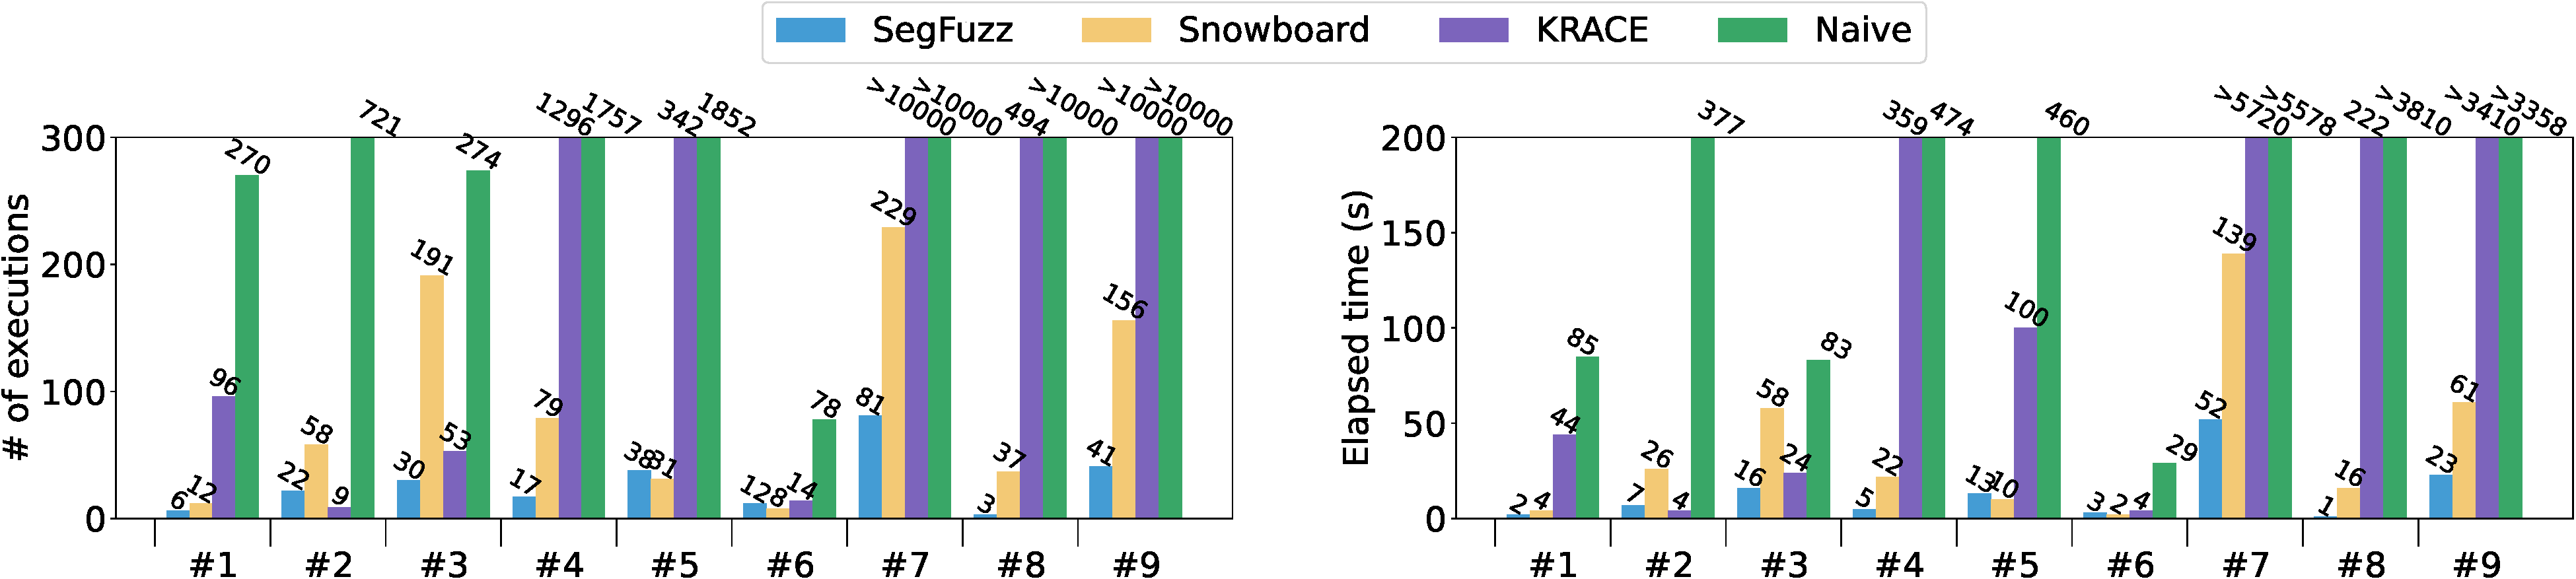
\includegraphics[width=0.5\linewidth]{fig/comparison_graph_execution-crop.pdf}}
% \subfloat[First.]{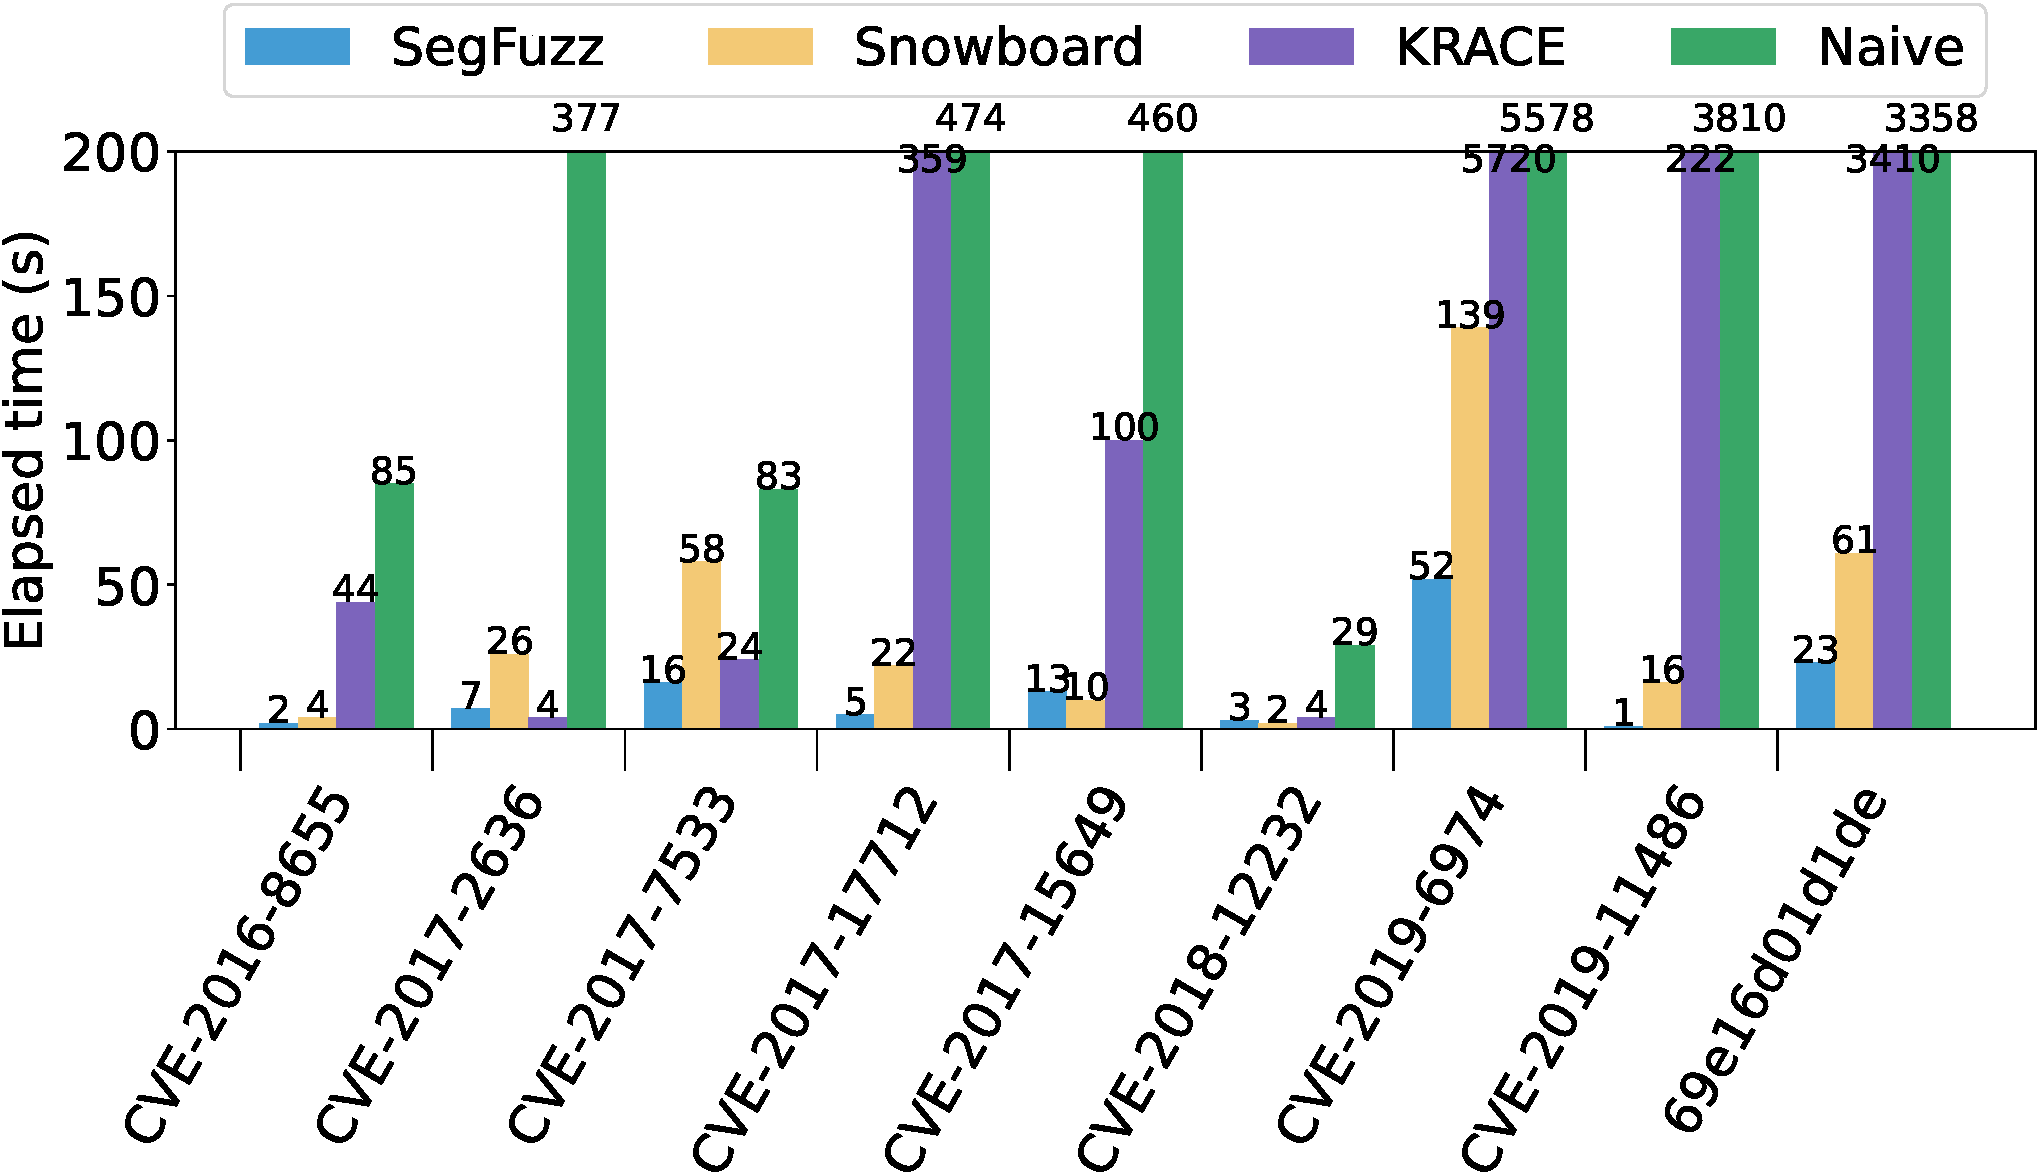
\includegraphics[width=0.5\linewidth]{fig/comparison_graph_time-crop.pdf}}\\
% \end{figure*}

%
One could argue that even if interleaving segment coverage is
informative to describe offending thread interleavings, 
its search space is too large to explore.
%informative in describing unique behaviors of offending thread
%interleavings, its search space is too large to explore, and thus, it
%is impractical.
%
However, it is tractable to run the mutation-based interleaving exploration
using \intcov.
To demonstrate this, we compare the mutation-based interleaving
exploration~\autoref{ss:scheduler} against various interleaving
exploration methods proposed in prior approaches.

\PP{Comparison target}
%
We compare \sys to state-of-the-art kernel concurrency fuzzers,
Snowboard~\cite{snowboard}, and KRACE~\cite{krace}.
%
Unfortunately, we cannot directly run Snowboard and KRACE for the
comparison study; KRACE is implemented only for file systems, and
Snowboard runs based on the binary translation of QEMU, 

%
Therefore, we implement their approaches on the multi-thread fuzzing
phase~(\autoref{sss:multithreadfuzzing}) of \sys by applying 1) the
random delay injection scheme of KRACE, and 2) the
enforcing-single-interleaving-order scheme used by Snowboard.
%
In addition to them, we also compare with the kernel scheduler 
(\ie, no thread scheduling control applied) as the naive baseline.

% %
% Arguably, the most straightforward metric to compare fuzzing
% techniques is the elapsed time until concurrency bugs are discovered.
% %
% However, the elapsed time heavily depends on the randomness;
% \dr{because a fuzzer generates an input program very randomly, it is
%   possible that one fuzzer quickly generates an input program that
%   causes a concurrency bug, while another fuzzer takes very long time
%   to generate the input program}.

% In order to minimize the impact of the randomness and to concentrate
% on the performance impact of scheduling mechanisms, we predefine a
% multi-thread input as shown in \autoref{fig:multithreadinput}, and let
% a fuzzer repeatedly execute the given multi-thread input without
% generating new inputs nor mutating syscalls in the given input.

% In addition, previous fuzzing approaches

\PP{Result}
%
\autoref{fig:eval:comparison-execution} and
\autoref{fig:eval:comparison-time} show the comparison result.
%
In these figures, \texttt{\sys}, \texttt{Snowboard}, and
\texttt{KRACE} display the number of executions and the elapsed time
taken by their corresponding works, and \texttt{Naive} corresponds to
the kernel scheduler without any thread scheduling control enabled.
%
%
In \texttt{Naive}, we can identify the difficulty of discovering
varies from a bug to a bug.
%
For example, CVE-2018-12232 appears as the easiest concurrency bug to
discover since it can be discovered within 78 executions even with the naive kernel scheduler.
%
On the other hand, the kernel scheduler fails to discover three
concurrency bugs, CVE-2019-6974, CVE-2019-11486, and
\texttt{69e16d01d1de} within 10K times of executions.
%
Regardless of the varying difficulty, \sys can discover all of
concurrency bugs within a short time.
%
\sys can discover given concurrency bugs within just 26.8 runs
(ranging from 3 to 81) and 13 seconds (ranging from 1 to 52) on
average.
%
Whereas, Snowboard discovers concurrency bugs within 89 runs (ranging
from 8 to 229 runs) and 37.5 seconds (ranging from 2 to 139) on
average, and KRACE discovers them, if successful, within 329.1 runs
(ranging from 9 to 1296) and 107 seconds (ranging from 4 to 359) on
average.  Moreover, KRACE even suffers from discovering CVE-2019-6974
and \texttt{69e16d01d1de}.

In summary, we confirm that the \sys's mutation-based 
interleaving exploration exhibits superior performance by 
quickly navigating the search space even if \intcov 
constructs more complex search space than the alias coverage.

\subsection{Performance characteristics of \sys}
\label{ss:characteristics}

In this subsection, we analyze various performance characteristics of
\sys to comprehend how our approach affects the fuzzing process.
%
\subsubsection{All-inclusive evaluation}
\label{sss:allinclusive}

Here, we provide performance characteristics of the whole \sys.


\PP{Coverage growth.}
%
\begin{figure}[t]
  \centering
  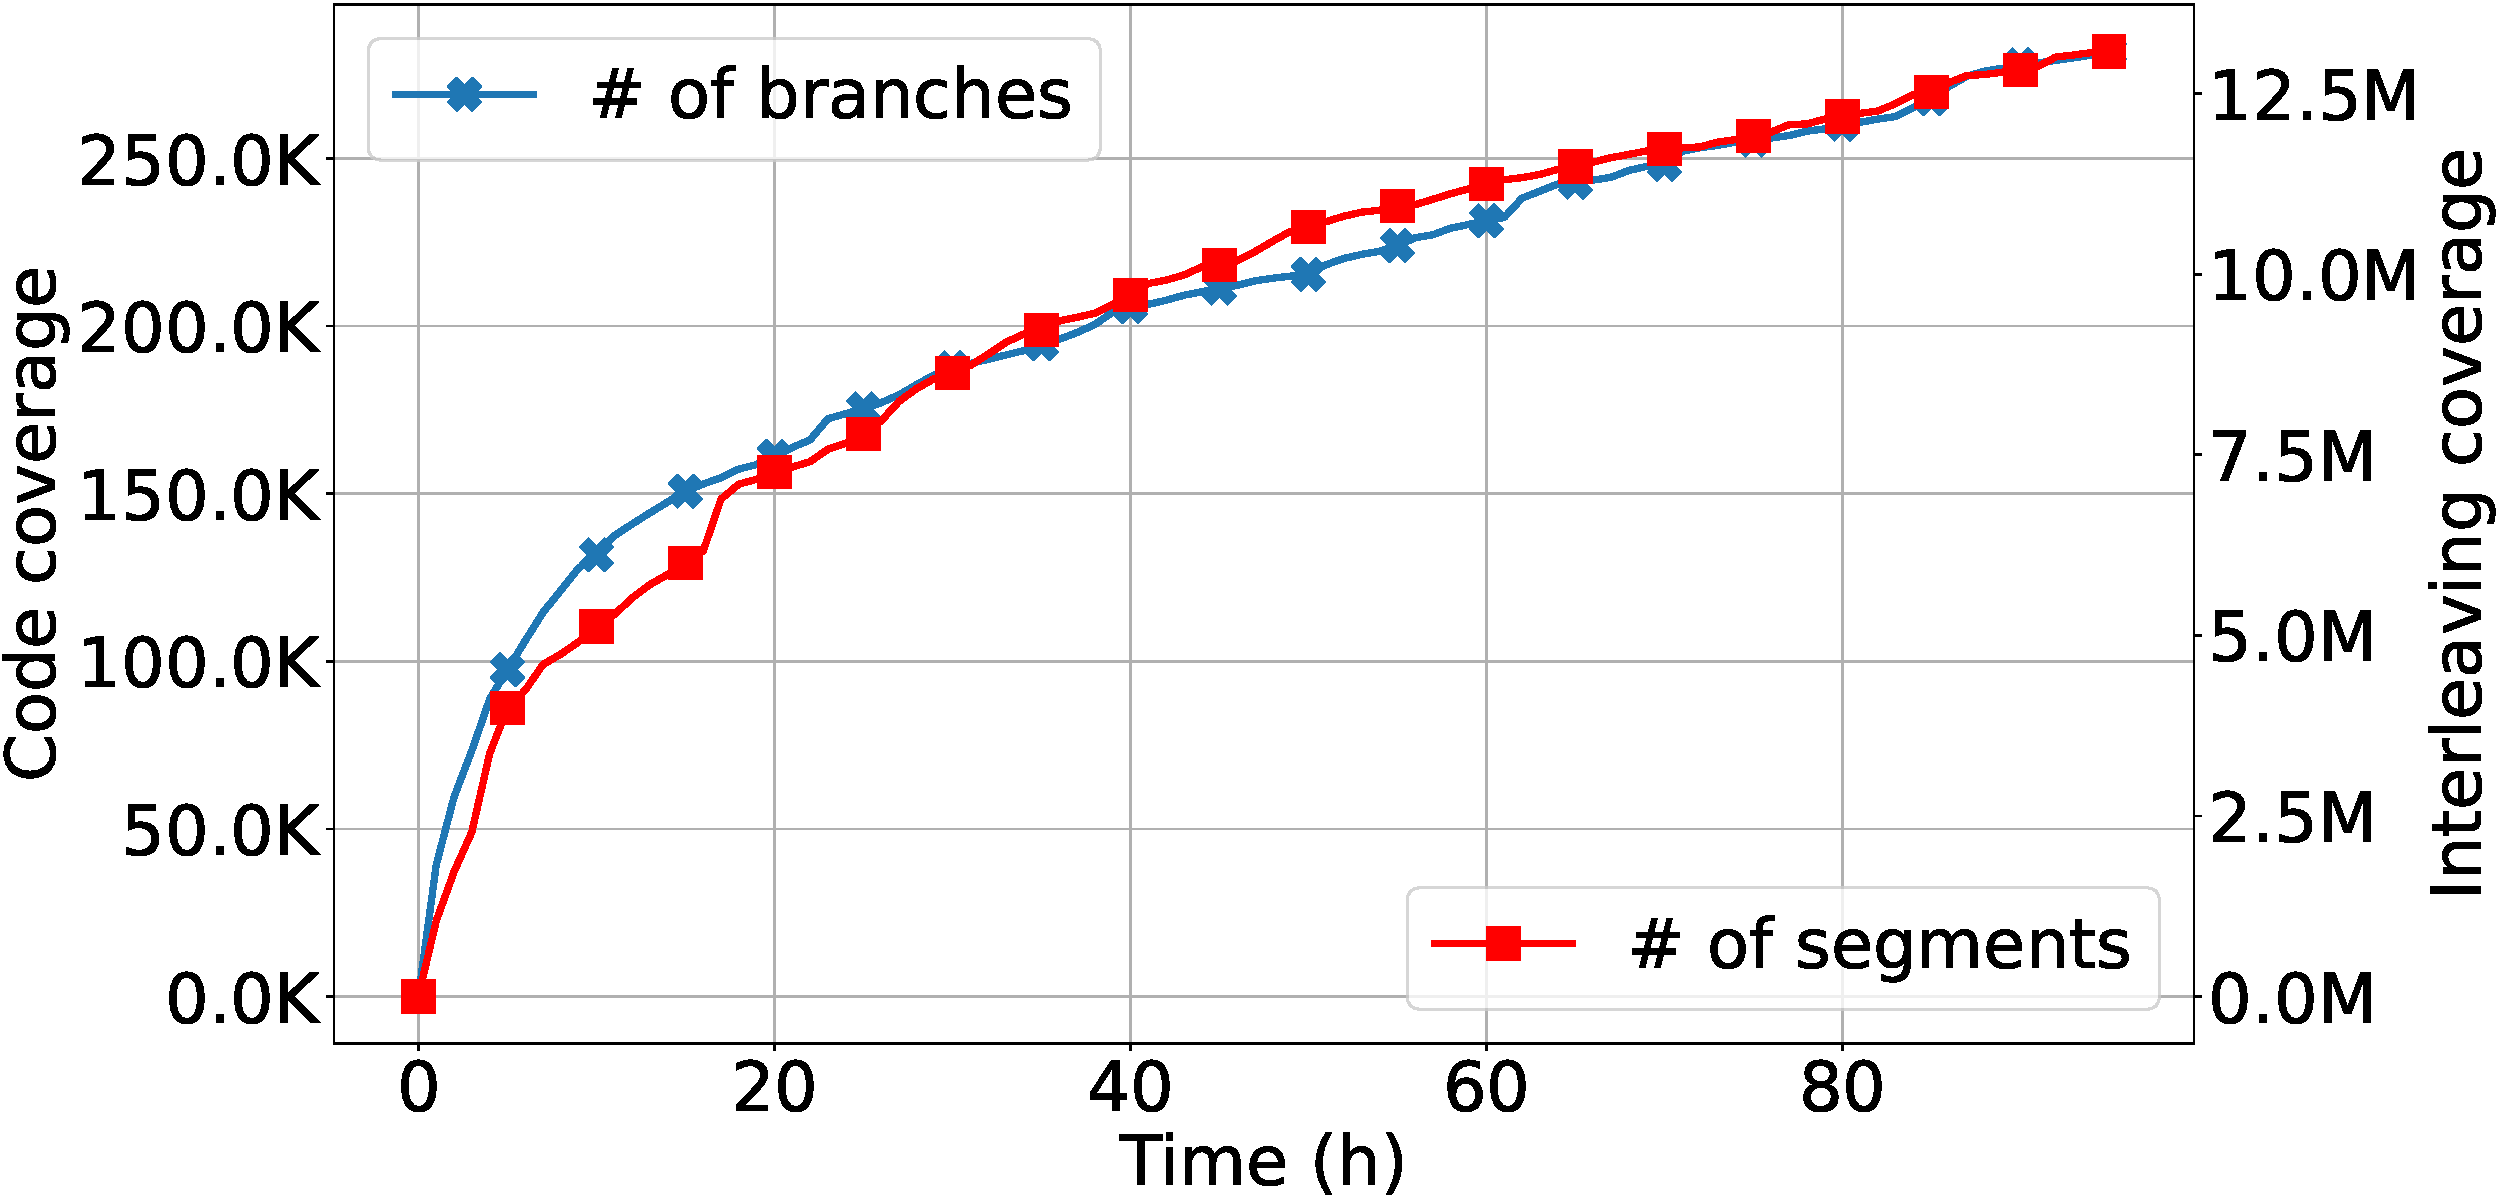
\includegraphics[width=0.9\linewidth]{fig/coverage_graph-crop.pdf}
  \caption{Coverage growth of \sys.}
  \label{fig:eval:coverage}
  \vspace{-5pt}
\end{figure}
%
Since coverage metrics are the paramount performance metric of
fuzzing, we measure the coverage growth for both code coverage (\ie,
the number of taken branches) and interleaving coverage (\ie, the
number of observed interleaving segments) during 100 hours of fuzzing.

As shown in \autoref{fig:eval:coverage}, there is a notable difference
in scale between code coverage (a line denoted by \texttt{Branch}) and
interleaving coverage (a line denoted by \texttt{Interleaving segment}).
%
While the number of taken branches just reaches to 300K, the number of
interleaving segments is over 20M. Thus, the scale of interleaving
coverage is more than 66 times of code coverage.
%
As a consequence, storing interleaving segment coverage consumes more
memory than storing branch coverage.
%
In our implementation, both branch coverage and interleaving segment
coverage are represented as hash tables where each element is 8
bytes. Therefore, storing interleaving segment coverage consumes about
180\MB while storing branch coverage requires 2\MB.
%
We can consider this result as a well-known space-time
tradeoff~\cite{spacetimetradeoff}; we invest \textit{more memory} to
discover concurrency bugs \textit{faster}.
%
% In addition, considering each VM is equipped with 8\GB memory, it is
% endurable for the fuzzer to store interleaving segment coverage using
% 180\MB (or even using ten times of 180\MB).


\PP{Fuzzing throughput.}
%
\begin{table}[t]
  \small
  \centering
  \resizebox{0.65\linewidth}{!}{
\begin{tabular}{l l l}
  \toprule
  \sys & \texttt{Syzkaller} & \texttt{Syzkaller-memtrace} \\
  \midrule
  4.55 & 8.40 & 4.74 \\
  \bottomrule
\end{tabular}
}



% syzkaller: 30234
% syzkaller-memtrace: 17608
% c2fuzz: 16386


%%% Local Variables:
%%% mode: latex
%%% TeX-master: "../p"
%%% End:

  \caption{Fuzzing throughput (\# of exec/s) of \sys and
    \texttt{Syzkaller}. \texttt{Syzkaller-memtrace} indicates
    throughput of \texttt{Syzkaller} with memory access tracing
    enabled.}
  \label{table:throughput}
  \vspace{-5pt}
\end{table}
%
All \sys's mechanisms provide benefits in finding concurrency bugs
with a cost of additional overheads and throughput degradation.
%
To comprehend the trade-off, we measure the fuzzing throughput of \sys
and compare it with the \texttt{Syzkaller}'s throughput.
%
In order to experiment in the same environment, we measure throughput
with an empty set of seed. And because both \texttt{Syzkaller} and
\sys restart VMs after an hour of fuzzing, we measure throughput in an
hour of execution in order to eliminate noises caused by, for example,
VM rebooting or kernel crashes.



\autoref{table:throughput} shows the result. As expected, \sys shows
the lower throughput than \texttt{Syzkaller}. In particular, the
\sys's throughput is about 54\% of the \texttt{Syzkaller}'s
throughput.
%
To further understand why the \sys's throughput is degraded, we
additionally measure throughput of \texttt{Syzkaller} while tracing
memory accesses (through instrumentation described in
\autoref{ss:instrumentation}), but not making use of it.
%
As shown in the \texttt{Syzkaller-memtrace} column in
\autoref{table:throughput}, it shows the throughput similar to that of
\sys; the \texttt{Syzkaller-memtrace}'s throughput is just 4.1\%
higher than the throughput of \sys.
%
These results indicate that the throughput of \sys is mainly degraded
by the heavy instrumentation to trace memory accesses.
%
However, as KRACE~\cite{krace} states, it can be understandable as the
cost for the high input quality.
%
In the fuzzer's perspective, while tracking memory accesses has
negative impacts on throughput, it provides a higher chance for a
fuzzer to execute more interesting inputs (\ie, interesting thread
interleaving) and not to waste computing resources.
%
The effectiveness of high input quality is more pronounced in
\autoref{sss:interleavingsearch}, showing \sys can discover
concurrency bugs very quickly.




\PP{Per-input overhead}
%
\begin{table}[t]
  \centering
  \resizebox{\linewidth}{!}{
  \begin{tabular}{l l l l l l }
    \toprule
    & & \multicolumn{2}{c}{Comp. overhead~(\autoref{s:design})} & \multicolumn{2}{c}{Runtime overhead~(\autoref{s:impl})} \\
    \midrule
    Total & \thead{Exec.\\syscall} & \thead{Tracking\\coverage\\(\autoref{ss:coverage})} & \thead{Interleaving\\search\\(\autoref{ss:scheduler})} & \thead{Tracing\\accsses\\(\autoref{ss:instrumentation})}  & \thead{Thread\\scheduling\\(\autoref{ss:engine})}  \\
    \midrule
    267.2 & 107.6  & 8.9 & 17.2 & 90.7 & 42.8 \\
    \bottomrule
  \end{tabular}
}

% temporary
% c2fuzz
%  execute            241116156.29326048
%  mutate             17231640.620481927
%  post               8858728.732142856
% syzkaller           107640966.51956181
% syzkaller-memtrace  198337534.77521613

%%% Local Variables:
%%% mode: latex
%%% TeX-master: "../p"
%%% End:

  \caption{
    %
    Elapsed time (ms) for executing one multi-thread input. We
    decompose the elapsed time into the system call execution
    (\texttt{Exec. syscall}), \sys's computational overheads
    (\texttt{Comp. overhead}) and runtime overhead (\texttt{Runtime
      overhead}).}
  \label{table:elapsedtime}
  \vspace{-8pt}
\end{table}
%
In \sys, there are two types of overheads for executing a single
multi-thread input, \ie, computational overheads and runtime
overheads.
%
Specifically, computation overheads are caused by tracking
interleaving segment coverage after executing the
input~(\autoref{ss:coverage}), and calculating scheduling points
before executing the input~(\autoref{ss:scheduler}).
%
On the other hand, runtime overheads are caused by tracing memory
accesses~(\autoref{ss:instrumentation}) and controlling thread
scheduling~(\autoref{ss:engine}).
%
To closely examine these overheads, we measure the elapsed time for
executing a single multi-thread input, and break down the elapsed time
into time taken by each components.
%
For this measurement, we run 10 thousands times and take an average.




\autoref{table:elapsedtime} shows the result. When executing a single
input, the total elapsed time is 267.2ms.
%
During the execution, the part that took the longest time is executing
system calls; it takes 107.6ms.
%
However, overheads incurred by \sys is not negligible. Tracing memory
accesses~(\autoref{ss:instrumentation}) takes 90.7ms, and controlling
thread scheduling~(\autoref{ss:engine}) takes 42.8ms. These two
runtime overheads almost double the execution time, and are the main
cause of degrading the throughput of fuzzing as shown in the above.
%
In contrast, the total amound of time for computation is 26.1 (= 8.9 +
17.2)ms, and occupies approximately 9\% of the total elapsed time.
%
Accordingly, we can see that the computational overhead is relatively
small.



\subsubsection{Impact on coverage growth}
\label{sss:component}
%
Here, we present the impact of our design choices on both the
interleaving coverage growth and the code coverage growth.


\PP{Impact on interleaving exploration}
%
As the primiary purpose of this work is to effectively explore thread
interleavings, the \sys's approach~(\autoref{s:design}) should
contribute in effectively expanding the interleaving coverage.
%
To see how much \sys improves thread interleaving exploration, we
disable the thread scheduling control in the multi-thread fuzzing
phase of \sys, and measure the interleaving coverage.
%
The result is described in a line denoted by \texttt{Interleaivng
  segment w/o scheduling control} in \autoref{fig:eval:coverage}.
%
With the thread scheduling control disabled, \sys finds 29.1\% less
interleaving segment coverage during the same period.
%
As a consequence, we can concolude that our design choices
significantly improve in exploring thread interleavings.
%
% As a consequence, \sys can effectively discover concurrency bugs as
% shown in \autoref{ss:comparison}.



\PP{Impact on code exploration}
%
Since \sys invests the computing power to repeatedly execute a
multi-thread input (\ie, the multi-thread fuzzing phase), we expect
that \sys might explore code coverage less than the baseline
\texttt{Syzkaller}.
%
To see the difference of the code coverage exploration in \sys and
\texttt{Syzkaller}, we measure code coverage of \texttt{Syzkaller} and
illustrate it as a line denoted by \texttt{Branch (Syzkaller)} in
\autoref{fig:eval:coverage}.
%
As a result, \sys finds 3.2\% less code coverage compared to the
baseline \texttt{Syzkaller}.
%
While this is a definitely downside of \sys. However, considering the
huge benefit in exploring thread interleavings, we still believe that
this is marginal.





%%% Local Variables:
%%% mode: latex
%%% TeX-master: "p"
%%% End:

\section{Limitation and Discusssion}
\label{s:discussion}

\PP{}
%
% dr: size of the interleaving space

\PP{}
%
% dr: bug that are not captured using segment

\PP{}
%
% dr: more threads

%%% Local Variables:
%%% mode: latex
%%% TeX-master: "p"
%%% End:

\section{Related work}
\label{s:relwk}

For decades, immense efforts have been made to effectively discover
concurrency bugs. In this section, We describe prior efforts in three
categories, data race detection, controlled concurrency testing, and
fuzzing.


\PP{Data race detection}
%

\cite{lkmm, linuxmemorymodel}


\PP{Controlled concurrency testing}
%


\PP{Fuzzing}
%
Since a kernel is a security basis of most systems, eliminating bugs
in a kernel is a paramount task to provide reliable
services. Therefore, many fuzzing approaches have been proposed to
find out bugs as the first step towards eliminating them.
%

IMF~\cite{imf}

Syzkaller~\cite{syzkaller},

Moonshine~\cite{moonshine}

HFL~\cite{hfl}

Healer~\cite{healer} is

Janus~\cite{janus}

Hydra~\cite{hydra}


Although we adopt Syzkaller as its sequential mutation, 

\PP{Concurrency fuzzing}
%
To the best of our knowledge, Razzer~\cite{razzer} is the first
attempt to improve a fuzzing technique in discovering concurrency
bugs.
%
The main idea of Razzer is to guide


After Razzer, Krace~\cite{krace} asserts the necessity of a coverage
metric in the concurrency dimension. Krace defines alias coverage


MUZZ~\cite{muzz}


Snowboard~\cite{snowboard}



%%% Local Variables:
%%% mode: latex
%%% TeX-master: "p"
%%% End:

\section{Conclusion}
\label{s:conclusion}

% We proposed RAZZER, a fuzz testing tool tailored to find race
% bugs. It utilizes a static analysis to spot potential data race points
% to guide the fuzzer to identify races. Moreover, it modifies the
% underlying hypervisor to trigger a race deterministically. The
% evaluation of RAZZER demonstrates its strong capability to
% detect races. It has thus far detected 30 new races in the Linux
% kernel, and a comparison study with other state-of-the-art tools,
% specifically Syzkaller and SKI, demonstrates its outstanding
% efficiency to detect race bugs in the kernel.

% We perform in-depth studies of Linux kernel concurrency
% bugs and drive three requirements: comprehensiveness, pattern-
% agnostic, and conciseness. This work proposes AITIA to sat-
% isfy the three requirements. AITIA fully automates the process
% of identifying the root cause of kernel concurrency bugs re-
% ported from existing bug-finding systems and analyzes the
% root cause as a form of a causality chain. We evaluate AITIA
% on 22 real-world concurrency bugs and successfully diagnose
% six unfixed bugs using AITIA.


In this paper, we propose \sys, a novel and effective kernel
concurrency fuzzer.
%
The key improvement of \sys resides in 1) adopting informative
interleaving coverage called interleaving segment coverage, and 2)
speculative interleaving exploration by utilizing explored
interleaving coverage.
%
As a result, \sys has discovered \totalbugs previously-undisclosed
concurrency bugs, and a comparison study demonstrates that \sys
outperforms state-of-the-art concurrency fuzzers, showing the
effectiveness of \sys.



%%% Local Variables:
%%% mode: latex
%%% TeX-master: "p"
%%% End:

% \section{Acknowledgment}
\label{s:ack}

%%% Local Variables:
%%% mode: latex
%%% TeX-master: "p"
%%% End:


\balance
\bibliographystyle{abbrvnat}
\footnotesize
\setlength{\bibsep}{3pt}
\bibliography{p,sslab,conf}

\normalsize
\vfill\eject
\appendix
\section{Appendix}

\subsection{Virtual Machine Introspection}
\label{s:appendix:vmi}


As a hardware breakpoint does not distinguish the running context of a
kernel, if the context switch happens, a breakpoint may be hit by
another thread or an interrupt handler, making the execution out of
expectation.
%
The hypervisor recognizes a running context using \texttt{task_struct}
which holds the thread description, and the per-cpu
\texttt{preempt_count} variable indicating what context the thread is
in (\eg, a task context for running a syscall, or a hardIRQ context to
handle hardware interrupts).
%
If a breakpoint is hit by a context other than the fuzzer-controlled
thread, our hypervisor ignores it and keeps the breakpoint.



When the suspended thread already acquires a lock while the running
thread wants to hold the same lock, the whole execution cannot make a
progress, because our hypervisor forces the lock-holding thread to
suspend.
%
Therefore, our hypervisor inspects whether the running thread is going
to be blocked due to the lock contention, and if it is, our hypervisor
takes control from the running thread to the suspended thread.
%
Inspecting the lock contention is conducted by hooking lockdep
functions~\cite{lockdep} that are commonly called from synchronization
prmitives.
%
When the lockdep functions are called, our hypervisor determins
whether the running thread can make a progress through various
information such as the address of the synchronization primitive, and
operation type (\ie, lock, unlock, and trylock).


%%% Local Variables:
%%% mode: latex
%%% TeX-master: "p"
%%% End:


\end{document}

%%% Local Variables:
%%% mode: latex
%%% TeX-master: "p"
%%% End:
